\chapter{基于目标追踪的毫米波雷达点云的姿态识别方案}
本章提出了一种基于目标追踪的毫米波雷达点云姿态识别方案MR-PPFN(Millimeter Wave Radar ParallelPoseFusionNet),该方案解决传统点云姿态识别算法在多目标的复杂场景因点云数据的无序性、稀疏性和噪声等因素,无法有效提取出关键的特征信息,导致识别准确率较低的问题。
MR-PPFN是一种通用的姿态识别网络架构,其主要是由两个并行特征提取子网络、自适应特征融合层以及分类回归层构成。在本章中,将详细介绍MR-PPFN设计过程,通过与PointNet、PointNet++、PointCNN、SpiderCNN、DGCNN、RsNet、BILSTM等模型集成来研究目标特征对模型准确率的影响。此外,由于现有的毫米波雷达点云数据集缺乏目标点的相关信息,因此我们自建$xidianiot\_point\_cloud\_targets\_posture$数据集,我们首先对数据进行了可视化分析,然后采用滑动窗口技术进行预处理得到样本数据,从而方便输入模型进行实验。最后使用该数据集进行对比实验,验证了MR-PPFN方案的有效性。
\section{毫米波雷达点云姿态识别概述}
\subsection{毫米波雷达点云姿态识别问题分析}
毫米波雷达点云姿态识别的基本原理是通过毫米波雷达发射电磁波并接收回波,从而获取目标物体或表面的三维空间点云数据。而点云中包含了目标的空间位置、反射强度和速度信息等。通过对这些点云数据进行算法分析,可以识别目标物体的朝向和运动状态,从而进行姿态估计。然而传统的毫米波雷达点云姿态识别算法仅仅只是依靠点云来进行姿态估计,由于点云的无序性和稀疏性,往往无法有效提取出点云的全局和时序的特征信息,导致识别准确率显著降低。因此,需要一个更加有效的基于毫米波雷达点云的姿态识别方案,以克服毫米波雷达无法有效提取点云全局和时序特征的问题。
\subsection{基于目标追踪的姿态识别方案}
基于上述的问题分析,本章创新性地将目标追踪的结果与毫米波雷达的点云数据进行结合,提出一种基于MR-PPFN的毫米波雷达点云姿态识别方案,其整体的流程如图\eqref{fig:mr-ppfn structure strategy}所示。整个流程主要包括以下三个步骤:

\begin{figure}[htbp]
    \centering
    \includegraphics[width=0.95\linewidth]{imgs/mr-ppfn structure.pdf}
    \caption{基于mr-ppfn的毫米波雷达点云姿态识别方案}
    \label{fig:mr-ppfn structure strategy}
\end{figure}

(1)\textbf{数据采集}:采用IWR6843毫米波雷达和数据采集程序进行相关姿态的数据采集,并创建$xidianiot\_point\_cloud\_targets\_posture$数据集。

(2)\textbf{雷达信号处理}:雷达底板程序会对雷达的回波数据进行对应的信号处理得到相关姿态的点云数据和目标点数据。首先通过FFT运算,将时域信号转换为频域信号,从而提取目标的距离、速度和角度等信息。然后通过BW Filter,过滤掉环境部分的噪声与干扰,增强目标信号的清晰度和质量。之后再对信号进行STFT运算,通过使用时间滑动窗口,并分别对每个窗口内的信号进行FFT运算,分析得到信号的频率随时间的变化规律,从而辅助识别和跟踪动态目标。最后再通过扩展卡尔曼滤波器,在噪声环境中对目标的状态运动状态进行准确估计和跟踪,预测目标的运动轨迹,得到目标的信息。并根据检测到的距离、速度和角度信息,计算得到目标在三维空间中的坐标、速度、加速度等信息,并生成对应的点云数据,作为后续网络的输入。

(3)\textbf{姿态识别}:将连续帧数的点云数据及其对应的目标数据输入到MR-PPFN网络,通过两个并行的子网络进行特征提取,PointCloud-SubNet和Targets-SubNet分别提取点云和目标点的关键特征,然后采用自适应融合层进行特征融合,并通过全连接层实现进一步进行特征提取,最后通过Softmax得到最终的分类结果。                

\section{$xidianiot\_point\_cloud\_targets\_posture$数据集构建}
\label{sec:dataset-build}
\subsection{问题分析}
首先由于现有的公开姿态识别数据集大多聚焦于对单人、单场景的姿态动作的捕捉,而缺乏对复杂场景的点云数据的采集,导致在多人动作叠加或背景干扰时模型的识别能力会显著受限。其次是现有的公开数据集仅仅只提供了目标的点云数据,通常只包括点云的空间的位置信息,而缺乏点云的特征属性,如俯仰角度、速度、加速度、信噪比、多普勒等,并且还缺乏点云对应的目标点信息。针对以上两个问题,本文自建了$xidianiot\_point\_cloud\_targets\_posture$数据集,提供了超过51万帧的训练数据,并且数据源更加的丰富,不但包括简单的单人场景的姿态数据,还包括更加复杂的多人复杂场景的姿态数据,并且该数据集的一帧数据是由目标点云数据和对应的目标点数据组成,点云数据中也包含了点云的特征属性。总的来说,$xidianiot\_point\_cloud\_targets\_posture$数据集增强了姿态识别场景的复杂性与多样性,并提供更丰富的训练数据。

\subsection{数据采集}
\label{sec:data-collection}
本章通过陕西省网络与系统安全重点实验室自研的物联网项目——校园安全防控系统进行点云和目标点数据的采集,构建相应的数据集。实验场地选择的是一间长度为9m、宽度3.6m,宽度为4.3m大小的房间,实验使用的德州仪器IWR-6843毫米波雷达设备如图\eqref{fig:IWR6843}所示,雷达的采集参数如雷达摆放的高度为2m,雷达摆放的位置如图\eqref{fig:experiment room and radar}所示,图\eqref{fig:pointcloud visuallization program}是雷达检测到目标人员对应的可视化程序的界面,图\eqref{fig:posture collection}是使用毫米波雷达分别采集摔倒、蹲下、走路、打架行为的示意图。

为了模拟现实生活中复杂的多人场景,首先是还原毫米波雷达在一段时间范围探测到目标数量变化的场景。进行单次采集的时候,多人在雷达探测的范围演示相应的动作,可以随机进出雷达探测的范围,这样可以真实还原现实场景中多人出入雷达的探测范围,人数不确定的情况。采集数据中包括了多人行走,多人打架等。其次是模拟了识别关键姿态动作时的背景干扰,比如说在打架的时候有人在行走等,增强了姿态识别场景的复杂性与多样性,提供更丰富的训练数据。
   
\begin{table}[htbp]
	\centering
	\tabcolsep=1cm
	\caption{雷达参数表}
	\begin{tabular}{cc}
			\toprule
			参数 & 数值 \\
			\midrule
			发射天线 & 4  \\
			接收天线 &3   \\
			ADC采样点数 & 128  \\ 
			开始频率 & 60GHz   \\
			空闲时间 & 10ns  \\
			每帧Chrip数 & 128 \\
			\bottomrule
	\end{tabular}
	\label{tab:radar params}
\end{table}

\begin{table}[htbp]
    \caption{实验采集数据参数}
	\label{tab:collection params}
	\begin{subtable}{.4\linewidth}
        \label{sample quantity}
		\centering
		\caption{采集数据样本量}
		\begin{tabular}{cc}
			\toprule
		    采集动作 & 采集样本数量  \\
			\midrule
			打架 & 4634 \\
			摔倒 & 141 \\
			蹲下 & 109 \\
			走路 & 4781 \\
			\bottomrule
		\end{tabular}
	\end{subtable}
	\begin{subtable}{.4\linewidth}
		\centering
		\caption{被试人员的信息}
		\begin{tabular}{ccccc}
			\toprule
			人员id &  性别 & 年龄 & 身高(cm) & 体重(kg)  \\
			\midrule
			1 & 男 & 25 & 175 & 65 \\
			2 & 女 & 22 & 160 & 50 \\
			3 & 男 & 28 & 180 & 70 \\
			4 & 女 & 24 & 165 & 55 \\
			5 & 男 & 26 & 178 & 68 \\
			6 & 女 & 23 & 158 & 48 \\
			7 & 男 & 27 & 182 & 72 \\
			8 & 女 & 25 & 162 & 52 \\
			9 & 男 & 29 & 185 & 75 \\
			10 & 女 & 26 & 168 & 58 \\
			\bottomrule
		\end{tabular}
	\end{subtable}  
\end{table}
\begin{figure}[htbp]
    \centering
    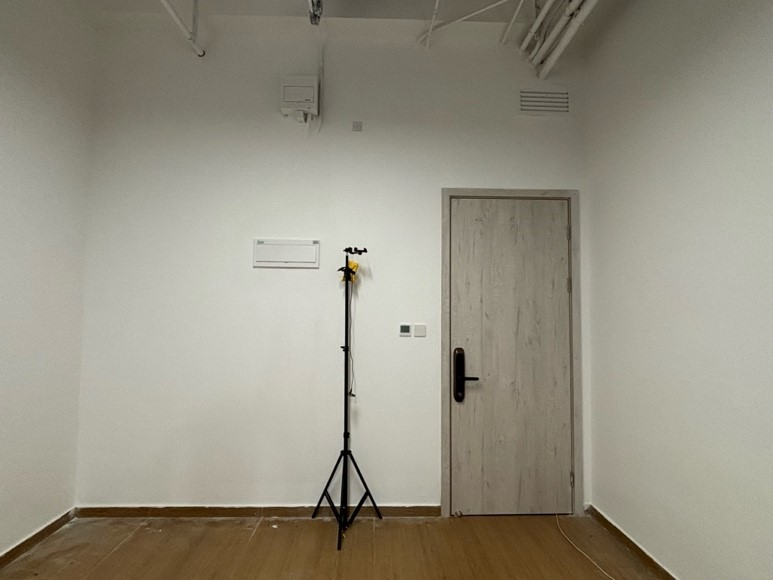
\includegraphics[width=0.5\linewidth]{imgs/experiment room and radar.jpg}
    \caption{实验房间和雷达摆放位置}
    \label{fig:experiment room and radar}
\end{figure}
\begin{figure}[htbp]
    \centering
    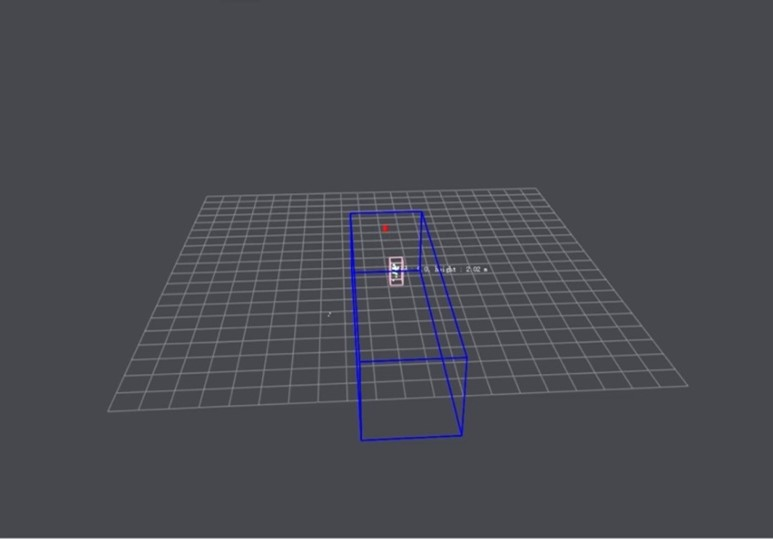
\includegraphics[width=0.5\linewidth]{imgs/pointcloud visuallization program.jpg}
    \caption{目标点云可视化程序}
    \label{fig:pointcloud visuallization program}
\end{figure}
\begin{figure}[htbp]
    \centering
    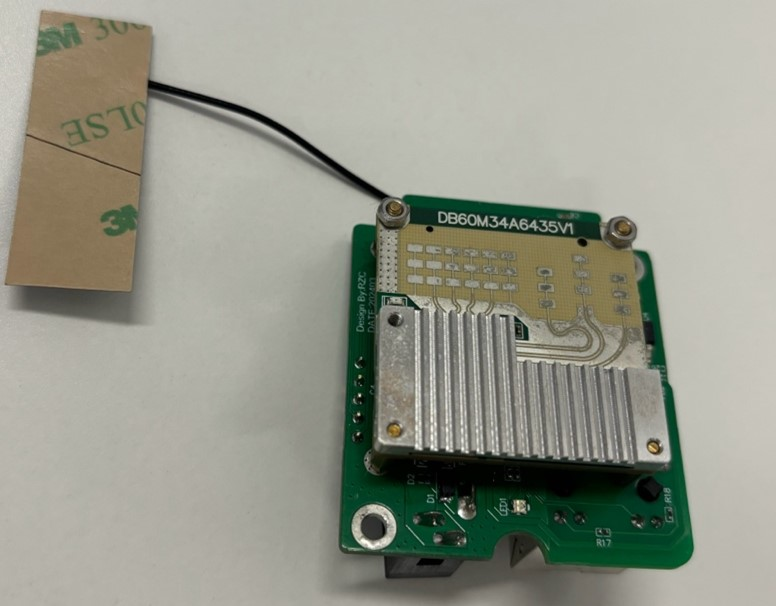
\includegraphics[width=0.5\linewidth]{imgs/mmware radar.jpg}
    \caption{IWR-6843毫米波雷达设备}
    \label{fig:IWR6843}
\end{figure}
\begin{figure}[htbp]
	\centering
	\subcaptionbox{摔倒\label{fig:falling}}{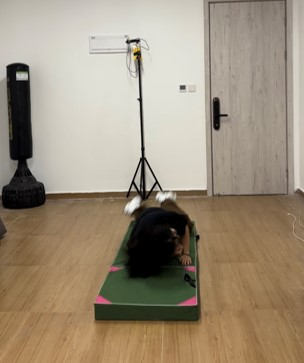
\includegraphics[width = 0.2\linewidth]{imgs/falling.jpg}}
	\subcaptionbox{蹲下\label{fig:squats}}{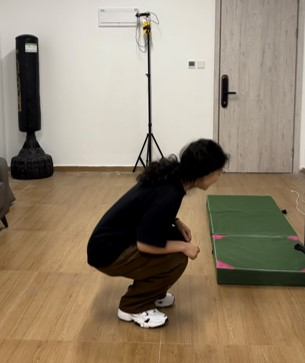
\includegraphics[width = 0.2\linewidth]{imgs/squats.jpg}}
	\subcaptionbox{走路\label{fig:walking}}{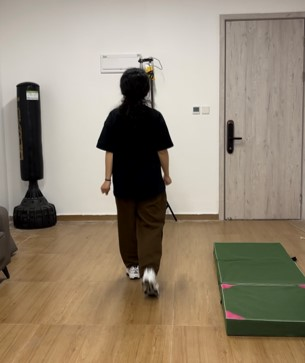
\includegraphics[width = 0.2\linewidth]{imgs/walking.jpg}}
	\subcaptionbox{打架\label{fig:fight}}{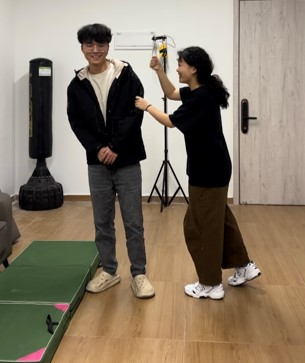
\includegraphics[width = 0.2\linewidth]{imgs/fight.jpg}}
	\caption{实验采集姿态示意图}
	\label{fig:posture collection}
\end{figure}
实验采集使用的毫米波雷达IWR-6843的参数设置如表\eqref{tab:radar params}所示,实验采集的参数如表\eqref{tab:collection params}所示,包括采集的样本数量和参与采集实验的被试者的信息。实验选择了10名被试,其中5名男性,5名女性,然后分别用毫米波雷达对这10名被试人员的四种姿态行为进行探测,包括打架(fight)、摔倒(falling)、蹲下(squats)、走路(walk)。本文定义连续15帧点云目标数据为一个样本,由于该研究是基于校园安全防控的背景,为了防止校园的霸凌行为,所以本数据集侧重对于打架行为的识别,总共采集了9665个样本,其中关键动作打架样本和最普通的动作行走样本数量相似。


\subsection{姿态点云数据可视化分析}
为了显示实验采集的每种姿态的点云与对应的目标点特征之间的联系,本节对不同姿态的动作进行可视化如\eqref{fig:posture_visualization}所示,分别显示了摔倒、蹲下、走路、打架四种姿态动作连续三帧点云以及对应目标点的位置和速度方向的变化。

\begin{figure}[htbp]
	\centering
	\subcaptionbox{摔倒\label{fig:falling_visualization}}{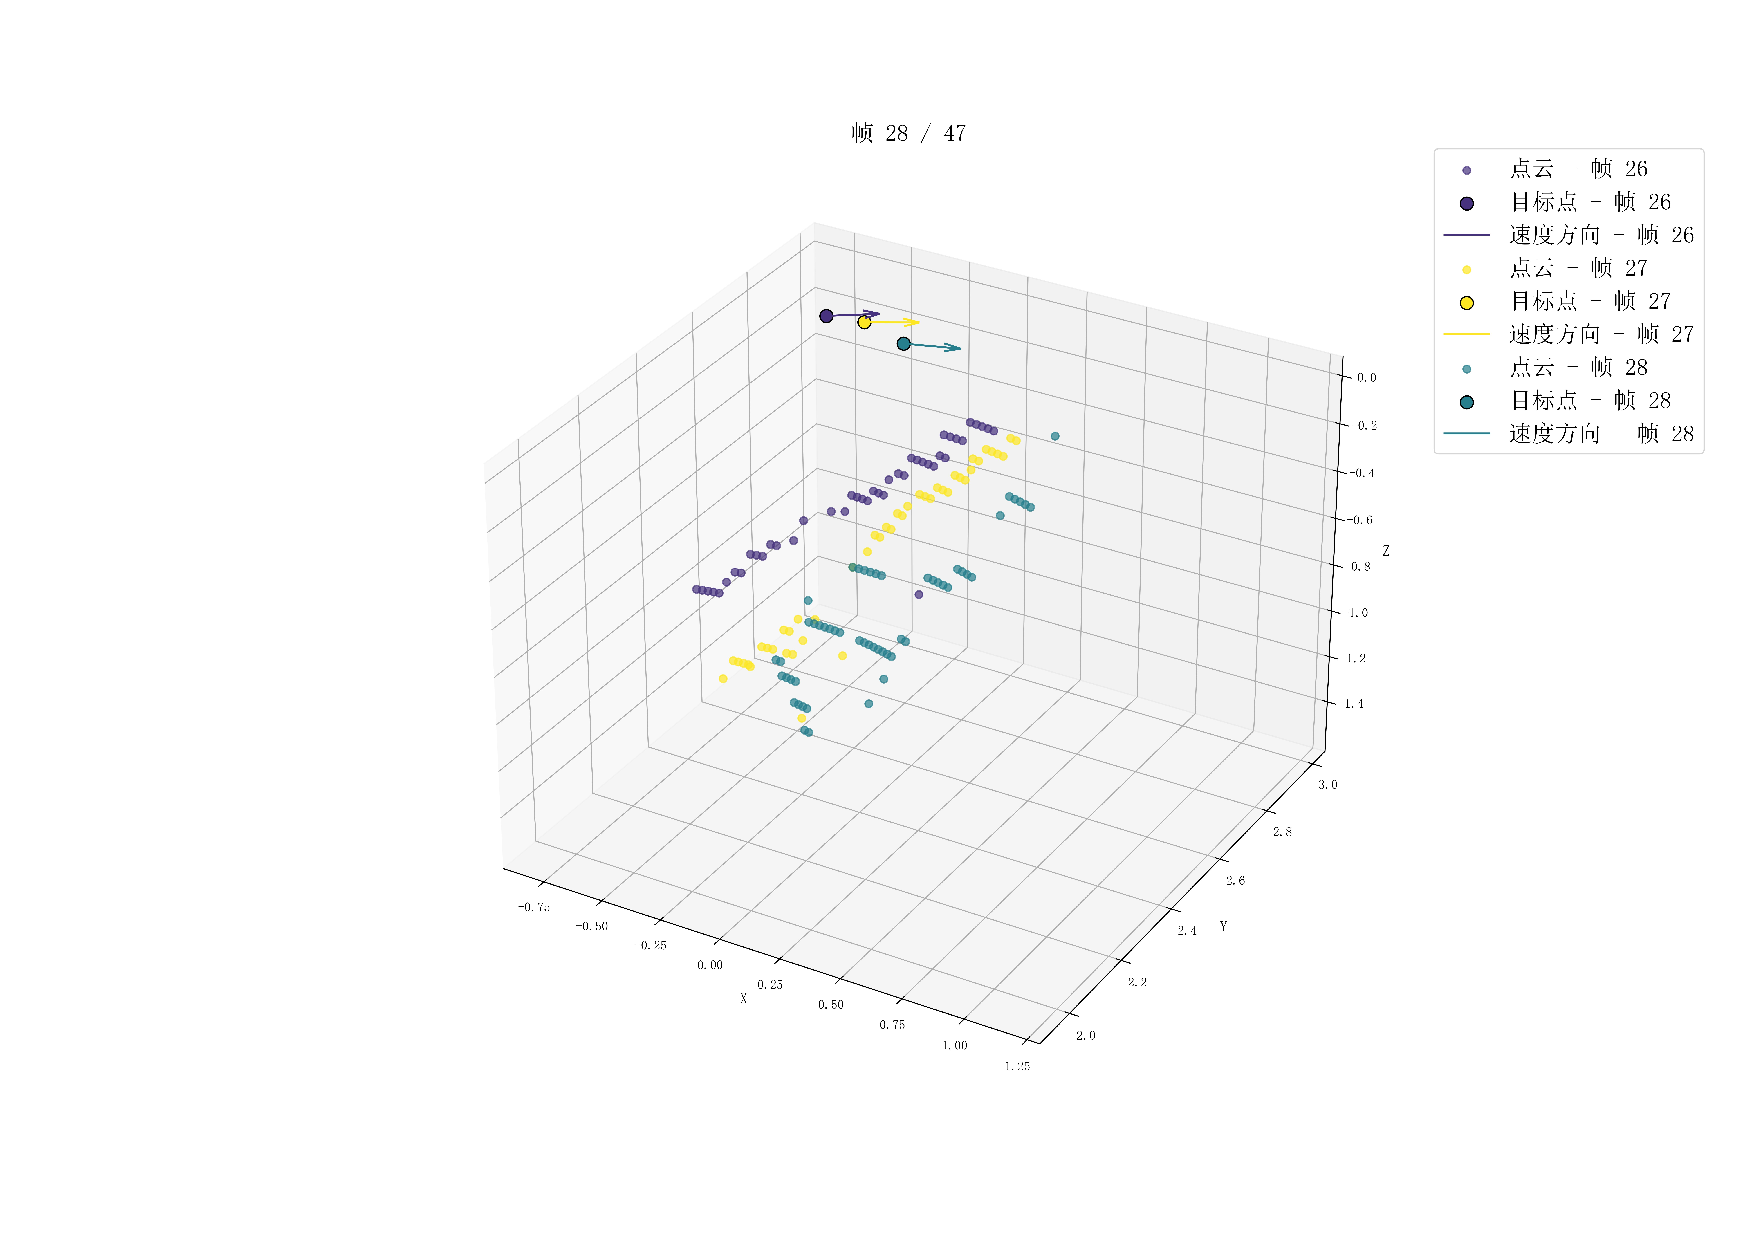
\includegraphics[width = 0.7\linewidth]{imgs/falling_visualization.pdf}}
	\subcaptionbox{蹲下\label{fig:squats_visualization}}{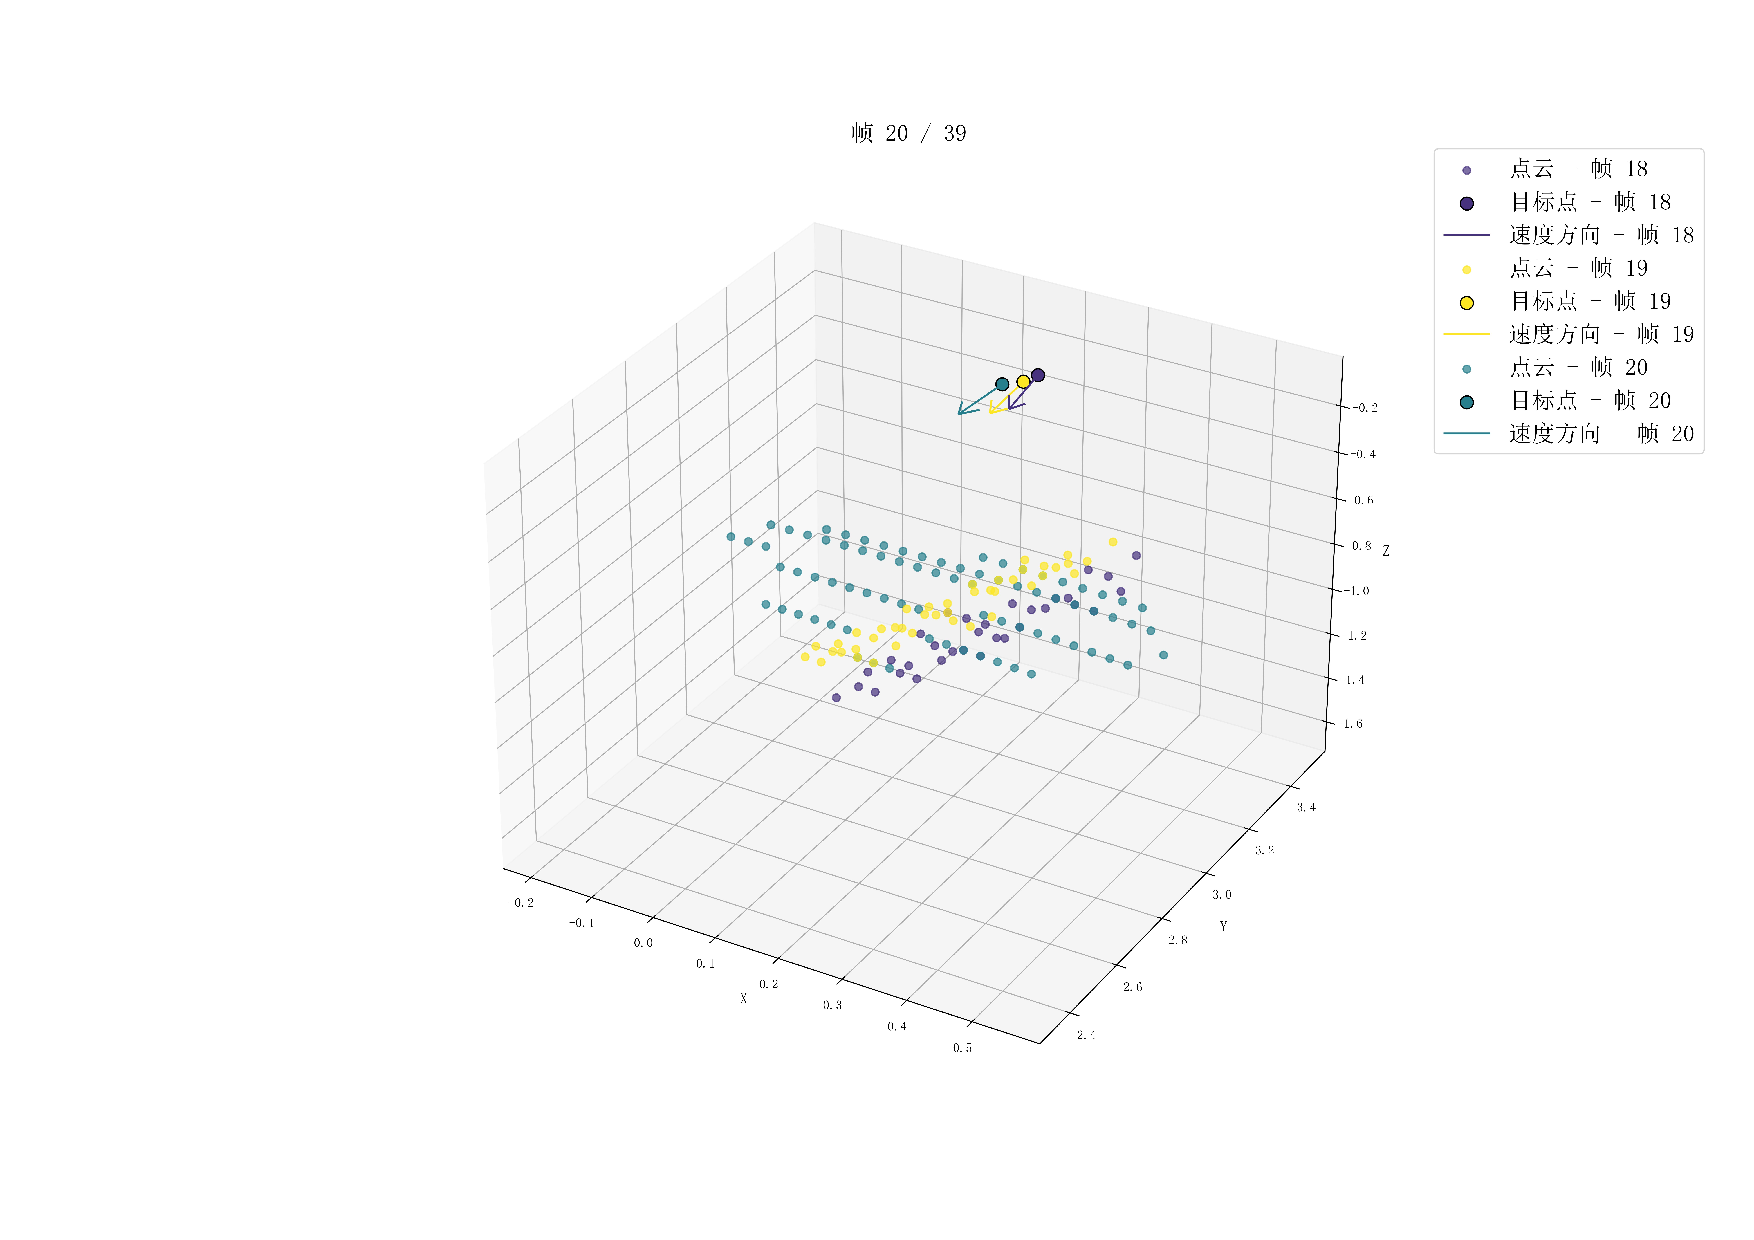
\includegraphics[width = 0.7\linewidth]{imgs/squats_visualization.pdf}}
    \subcaptionbox{走路\label{fig:walking_visualization}}{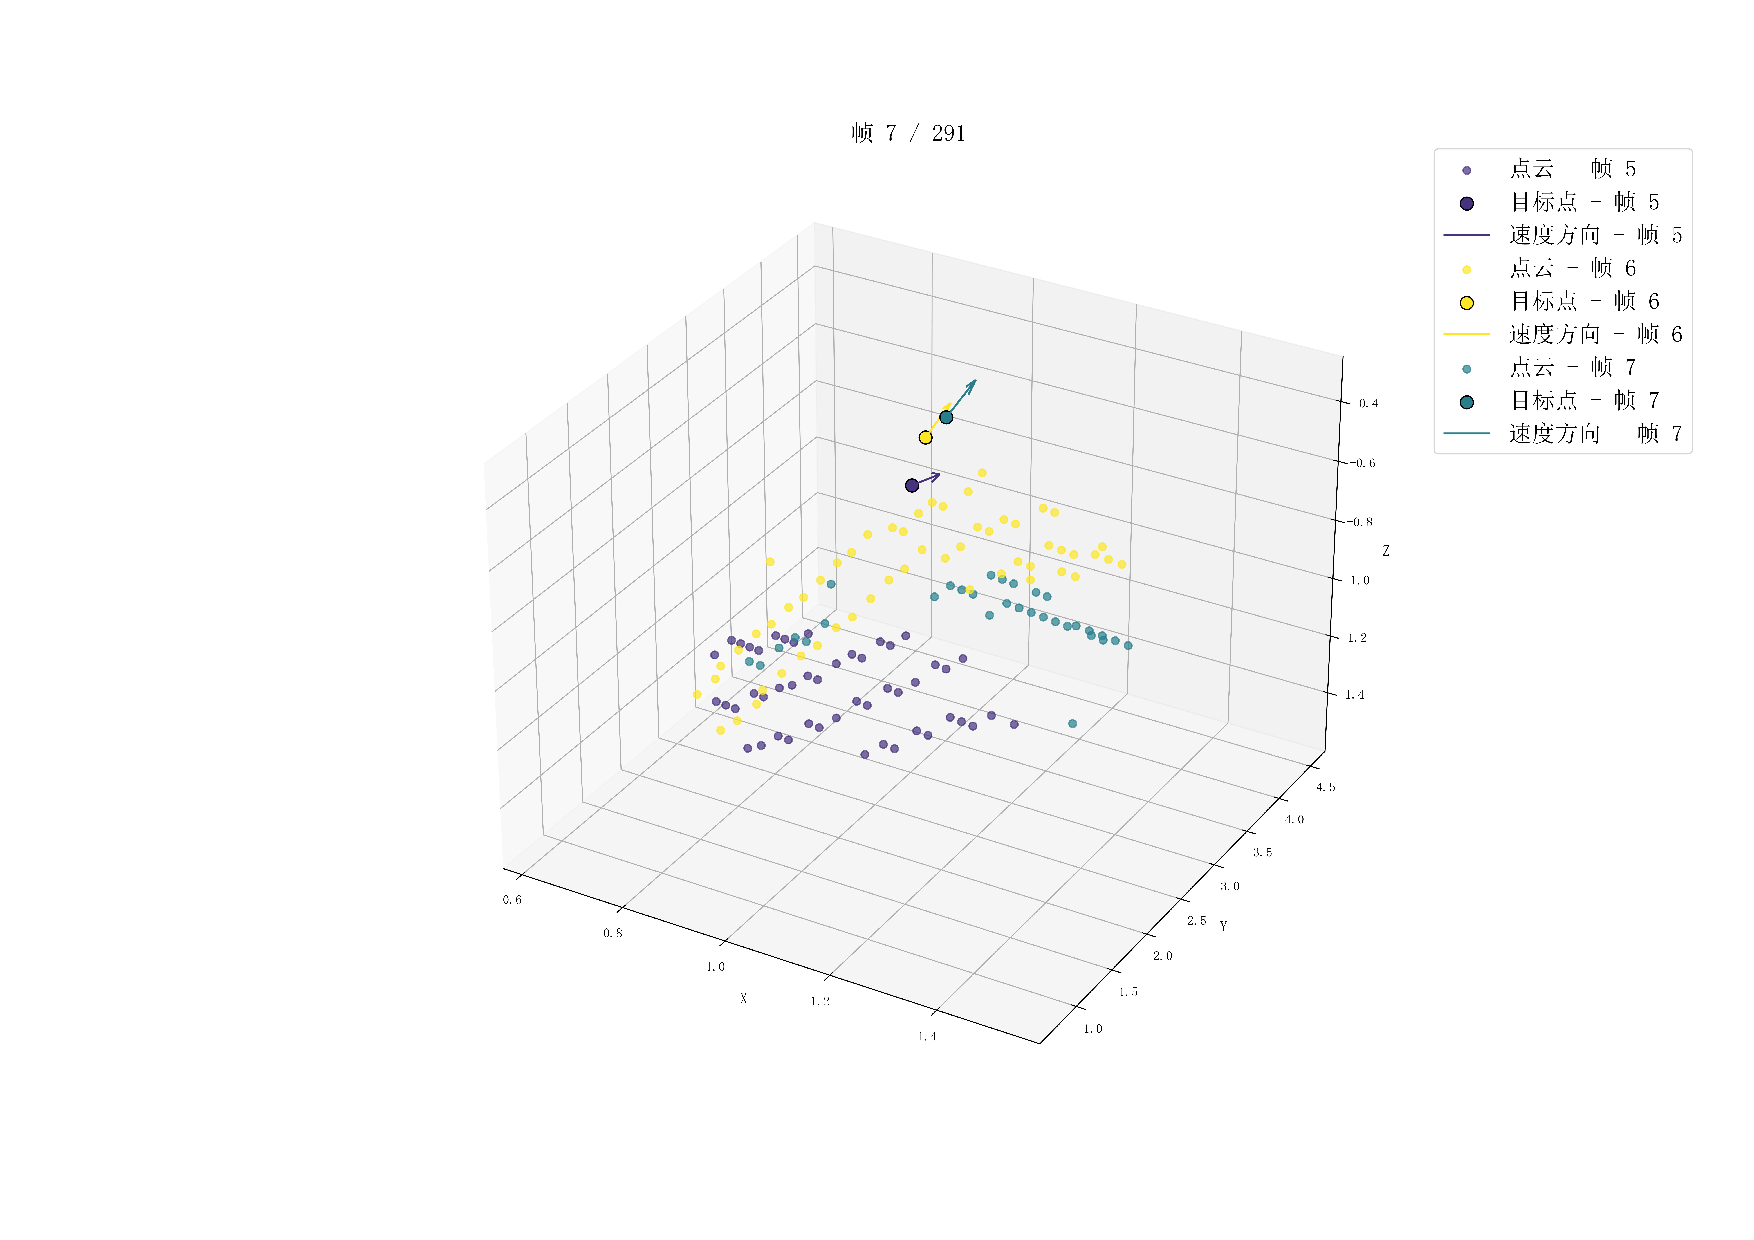
\includegraphics[width = 0.7\linewidth]{imgs/walking_visualization.pdf}}
\end{figure}

\begin{figure}[htbp]
    \ContinuedFloat
	\centering
    \subcaptionbox{打架\label{fig:fight_visualization_two_targets}}{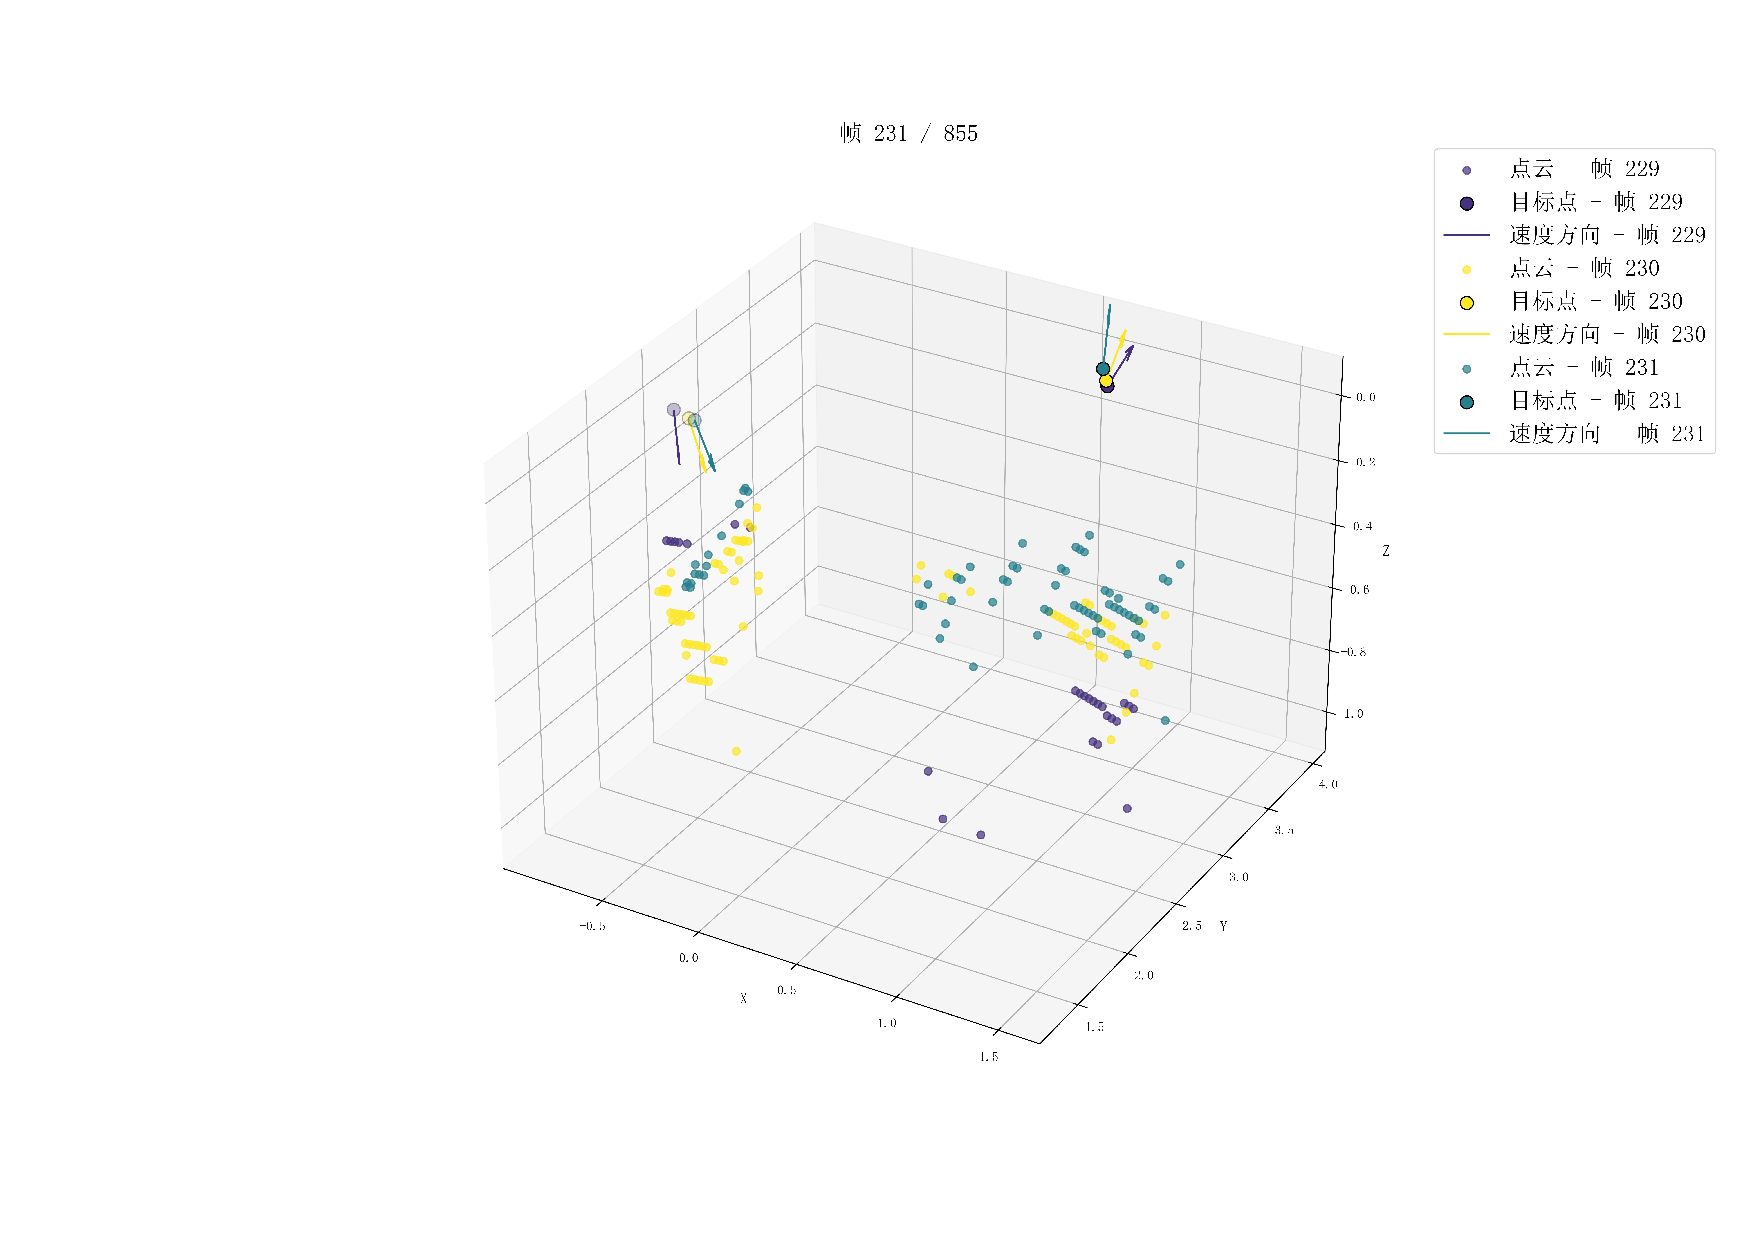
\includegraphics[width = 0.7\linewidth]{imgs/fight_visualization_two_targets.pdf}}
	\caption{实验采集四种姿态连续三帧数据的可视化示意图}
	\label{fig:posture_visualization}
\end{figure}

图\eqref{fig:Point Cloud  And Target Feature Analysis Over Frames}展示了点云特征和目标特征连续50帧的变化规律。
其中90\%Height Threshold是指在该帧中,90\%的点的高度低于或等于的阈值,其规定了点云中高度分布的上限,可以识别异常高的点和整体高度趋势,尤其在分析目标物体的垂直运动时可以更好地理解点云数据的高度特征。
同理90\%VelocityThreshold是指90\%的点的速度低于或等于的这个阈值,单位是(m/s),其规定了点云中速度分布的上限,便于识别异常快的点或整体速度趋势。Target Horizontal Offset是目标点的水平位移(m),其可以分析目标在水平方向上的运动轨迹,识别目标的移动模式或方向变化。Target Acceleration是目标点的加速度(m/s²),是指目标速度随时间的变化率,其可以分析目标的动态行为,例如:突然的加速度变化可能意味着目标正在快速启动或停止;持续的加速度可能表明目标在加速或减速。Target Height是目标点的高度(m),它反映了目标在垂直方向上的位置变化,起有助于分析目标的垂直运动,比如可以推测目标是否在上升或下降。Speed是指目标点的速度(m/s),有助于分析目标的运动特征。

图\eqref{fig:feature_analysis_falling}展示了摔倒姿态的点云和目标特征变化,其中90\%Height Threshold和Target Height曲线在前30帧较为稳定,但在30帧往后,开始持续明显下降,表示接近摔倒时整体高度降低,符合摔倒过程中身体逐渐接近地面的趋势。90\%VelocityThreshold和Target Acceleration曲线在摔倒开始和结束时有明显的波动,数值变化与前者相反,显著增加。Target Horizontal Offset保持稳定,表明摔倒过程中目标的横向移动不明显。总的来说,图中高度降低、速度增加和加速度变化反映了摔倒的特征,加速度和速度是在开始和结束时的剧烈变化反映了摔倒时的动态行为。
图\eqref{fig:feature_analysis_squats}展示了蹲下姿态的点云和目标特征变化,其各项特征的变化规律与摔倒动作十分的类似。但是蹲下动作的加速度和速度是在开始和结束时的变化的剧烈程度是低于摔倒动作的,因为摔倒动作这是一个无意识发生的动作,目标更类似一个自由落体的运动,这是区别这两个动作的关键特征。
图\eqref{fig:feature_analysis_walk}展示了走路姿态的点云和目标特征变化,其中除了曲线Target Horizontal Offset在水平偏移逐渐下降,说明目标在水平方向上有持续的移动,而其他特征曲线保持较稳定的状态。
\eqref{fig:feature_analysis_fight_two_targets}



\begin{figure}[htbp]
	\centering
	\subcaptionbox{摔倒\label{fig:feature_analysis_falling}}{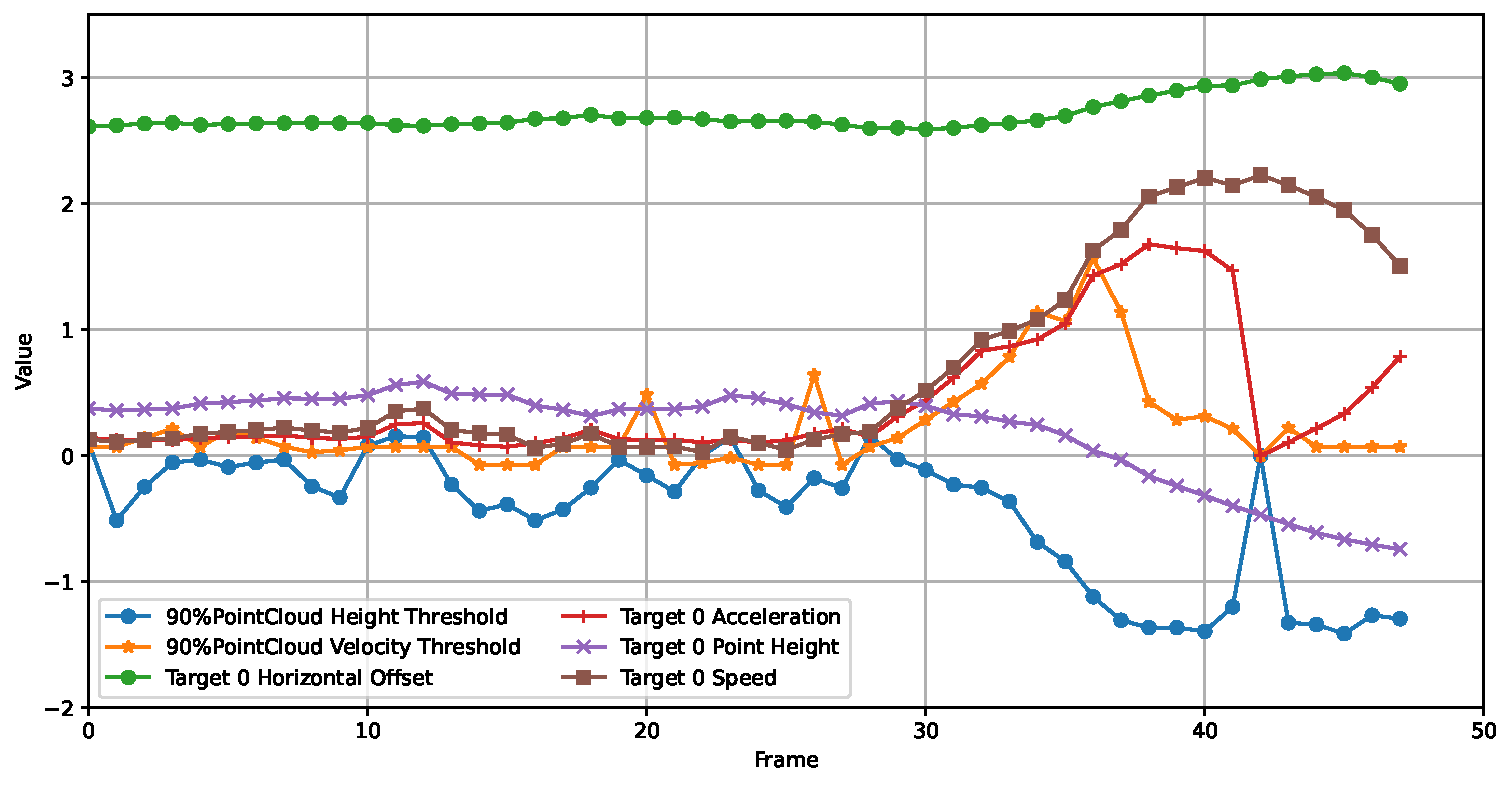
\includegraphics[width = 0.8\linewidth]{imgs/feature_analysis_falling.pdf}}
	\subcaptionbox{蹲下\label{fig:feature_analysis_squats}}{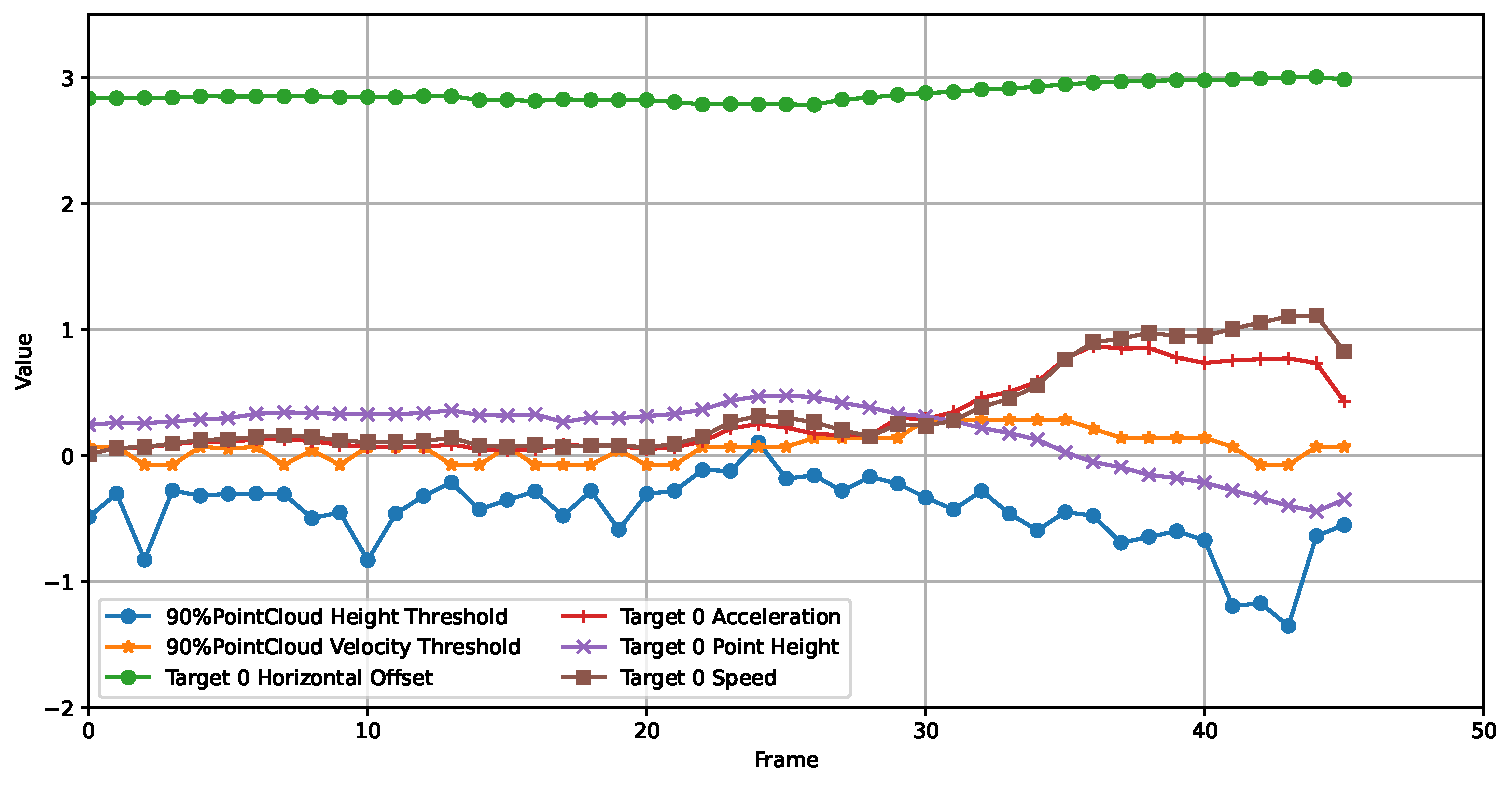
\includegraphics[width = 0.8\linewidth]{imgs/feature_analysis_squats.pdf}}
    \subcaptionbox{走路\label{fig:feature_analysis_walk}}{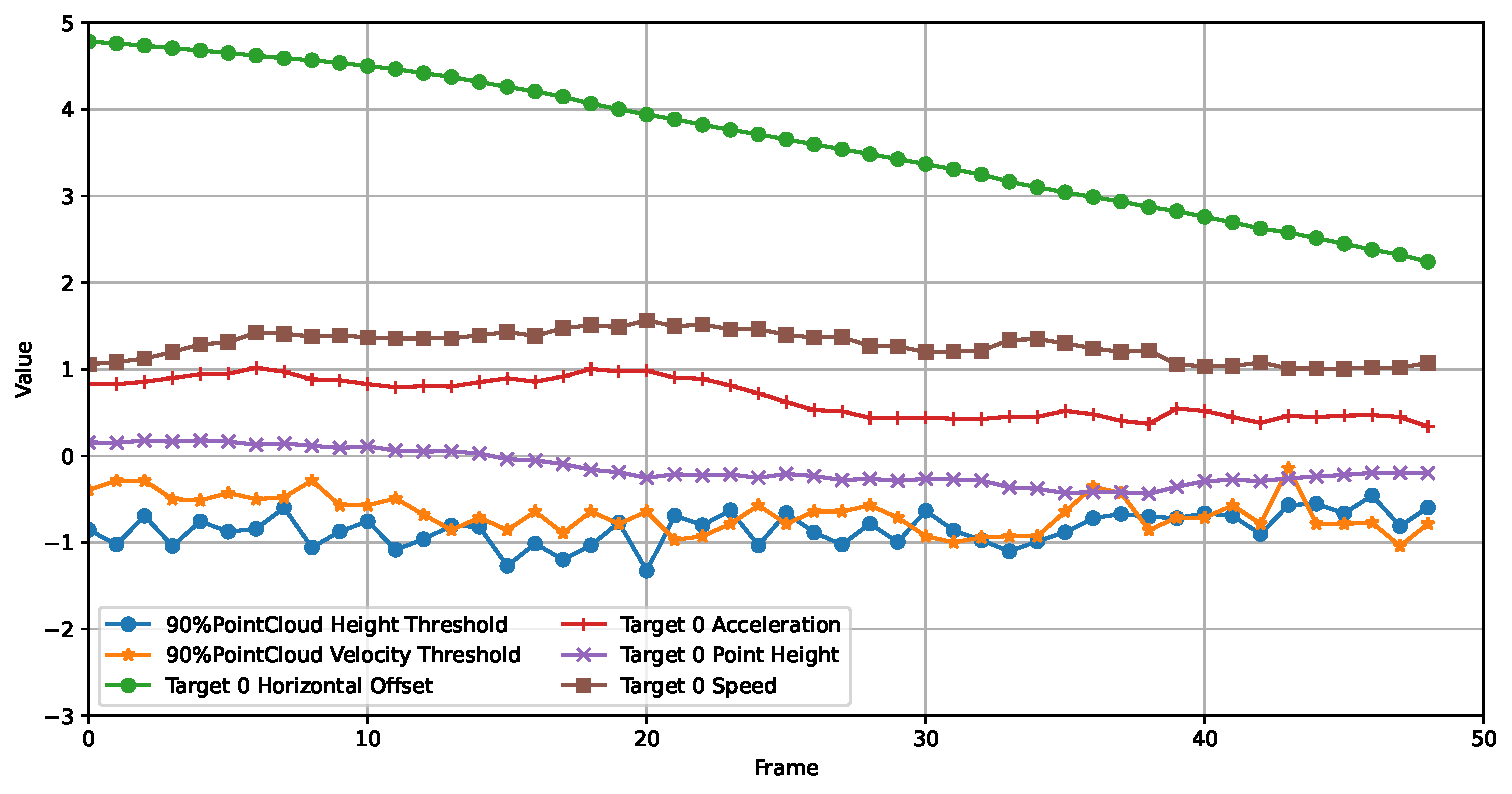
\includegraphics[width = 0.8\linewidth]{imgs/feature_analysis_walk.pdf}}
\end{figure}

\begin{figure}[htbp]
    \ContinuedFloat
	\centering
    \subcaptionbox{两个目标打架\label{fig:feature_analysis_fight_two_targets}}{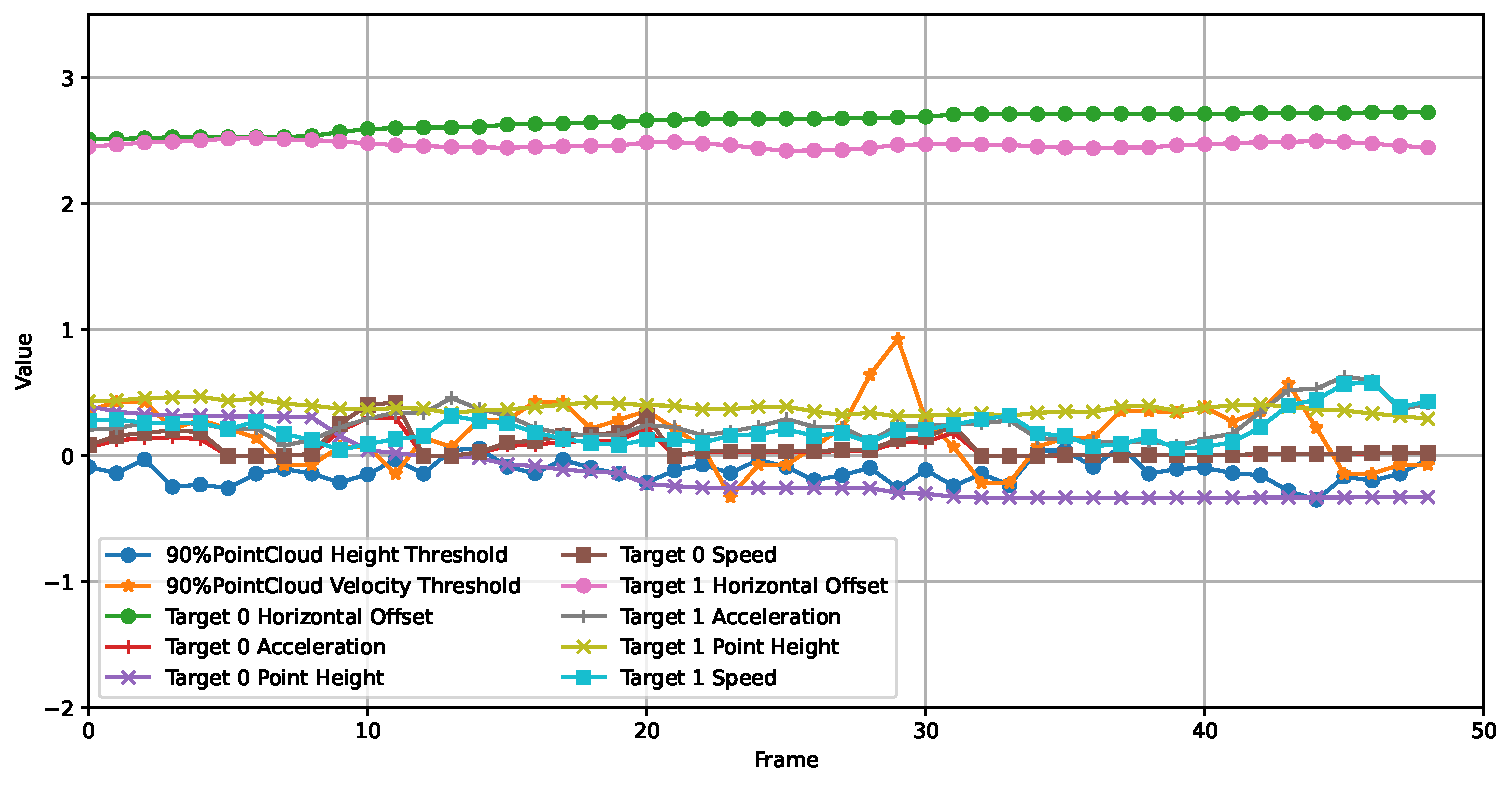
\includegraphics[width = 0.8\linewidth]{imgs/feature_analysis_fight_two_targets.pdf}}
	\caption{逐帧点云和目标点特征折线图}
	\label{fig:Point Cloud  And Target Feature Analysis Over Frames}
\end{figure}
 
\subsection{数据预处理}
\label{subsec:data preprocessing}
首先对点云目标数据格式进行定义,假设一帧点云数据的点云数量为 $n$,探测到的目标数目为 $m$。定义数据帧为:
\begin{equation}
    DataFrame = \{\mathbf{P},\mathbf{F}, \mathbf{T}\}
\end{equation} 
其中,点云数据 $\mathbf{P}$ 、点云属性$\mathbf{F}$和目标特征 $\mathbf{T}$ 分别定义为:
\begin{equation}
    \mathbf{P} = \begin{pmatrix}
        x_1 & y_1 & z_1 \\
        x_2 & y_2 & z_2 \\
        \vdots & \vdots & \vdots \\
        x_n & y_n & z_n
    \end{pmatrix}
\end{equation}
\begin{equation}
    \mathbf{F} = \begin{pmatrix}
        e_1 & s_1 & d_1 & r_1 & az_1 \\
        e_2 & s_2 & d_2 & r_2 & az_2 \\
        \vdots & \vdots & \vdots & \vdots & \vdots \\
        e_n & s_n & d_n & r_n & az_n
    \end{pmatrix}
\end{equation}
\begin{equation}
    \mathbf{T} = \begin{pmatrix}
        x_1 & y_1 & z_1 & a_{x_1} & a_{y_1} & a_{z_1} & v_{x_1} & v_{y_1} & v_{z_1} & id_1 \\
        x_2 & y_2 & z_2 & a_{x_2} & a_{y_2} & a_{z_2} & v_{x_2} & v_{y_2} & v_{z_2} & id_2 \\
        \vdots & \vdots & \vdots & \vdots & \vdots & \vdots & \vdots & \vdots & \vdots & \vdots \\
        x_m & y_m & z_m & a_{x_m} & a_{y_m} & a_{z_m} & v_{x_m} & v_{y_m} & v_{z_m} & id_m
    \end{pmatrix}
\end{equation}
$\mathbf{P}$中任意一个行向量为 $\mathbf{p}_i = (x_i, y_i, z_i)^T$ ,其代表一个点云的空间坐标。
$\mathbf{F}$中任意一个行向量为 $\mathbf{f}_i = (e_i, s_i, d_i, r_i, az_i)^T$,其表示一个点云的特征,分别是点云与毫米波雷达的俯仰角、信噪比、点云距离雷达的距离、多普勒和方位角。
$\mathbf{T}$中任意一个行向量为 $\mathbf{t}_j = (x_j, y_j, z_j, a_{x_j}, a_{y_j}, a_{z_j}, v_{x_j}, v_{y_j}, v_{z_j}, id_j)^T$ 其表示一个目标点的特征,分别是目标点的$x$,$y$,$z$ 轴的空间位置、加速度、速度和目标点的唯一标识。

首先是对目标特征进行特殊处理,由于探测到的目标点是会随时间发生变化的,为了方便输入到深度学习模型进行训练,将目标特征进行重新调整。一帧点云数据中,$m$是目标数量,$j$ 是目标特征数。将目标数据$\mathbf{T}$中任意一个行向量为 $\mathbf{t}_j$
拓展为维度为 $m \times j$的矩阵,拓展的部分使用零来填充,可以表示为:

\begin{equation}
    \mathbf{T}_{\text{extend}} = \begin{pmatrix}
        \mathbf{t}_1 & \mathbf{t}_2 & \cdots & \mathbf{t}_m \\
        \mathbf{0} & \mathbf{0} & \cdots & \mathbf{0} \\
        \vdots & \vdots & \ddots & \vdots \\
        \mathbf{0} & \mathbf{0} & \cdots & \mathbf{0}
    \end{pmatrix}
\end{equation}

本文采用滑动窗口算法将$xidianiot\_point\_cloud\_targets\_posture$数据集的数据处理成多个样本,窗口大小为$W$,步长为$S$(单位/帧)。定义一个样本为连续$W$的所有帧的集合,一个样本汇聚点云的数量为$p_{num}$,可以将一个样本的点云数据表示为:
\begin{equation}
    \mathbf{P}_{\text{raw}} = \begin{pmatrix}
        x_1 & y_1 & z_1 \\
        x_2 & y_2 & z_2 \\
        \vdots & \vdots & \vdots \\
        x_{p_{num}} & y_{p_{num}} & z_{p_{num}}
    \end{pmatrix}
\end{equation}
并且为了方便输入到模型进行处理,将每个样本的点云的数量统一调整到$N$,表示为:
\begin{equation}
    \mathbf{P}_{\text{sample}} = \begin{pmatrix}
        x_1 & y_1 & z_1 \\
        x_2 & y_2 & z_2 \\
        \vdots & \vdots & \vdots \\
        x_{p_{N}} & y_{p_{N}} & z_{p_{N}}
    \end{pmatrix}
\end{equation}
具体调整策略的算法如\eqref{alg:adjust_pointcloud}所示。
调整后的点云数据$\mathbf{P}_{sample}$的维度为$N \times 3$,其中$3$是每个点云数据的特征维度(点云的空间位置坐标)。
而一个样本的目标特征数据表示为:
\begin{equation}
    \mathbf{T}_{\text{sample}} = \begin{pmatrix}
        \mathbf{T}_{\text{extend}, 1} & \mathbf{T}_{\text{extend}, 2} & \cdots & \mathbf{T}_{\text{extend}, W}
    \end{pmatrix}
\end{equation}
一个样本数据用向量$Sample$表示为:
\begin{equation}
    Sample = \begin{pmatrix}
        \mathbf{T}_{\text{sample}} \\
        \mathbf{P}_{\text{sample}}
    \end{pmatrix} 
\end{equation}
其中,$\mathbf{T}_{\text{sample}}$ 是样本的目标特征向量,$\mathbf{P}_{\text{sample}}$ 是样本的点云特征向量。

假设有$M$帧数据,总共样本的数量可以通过公式\eqref{eq:sample sum}计算得到,所有样本可以用公式\eqref{eq:sample total}表示。
\begin{equation}
    \label{eq:sample sum}
    \mathbf{sum} = \left\lfloor \frac{M - window\_size}{step} \right\rfloor + 1
\end{equation}
\begin{equation}
    \label{eq:sample total}
    Sample_{total} = \begin{pmatrix}
        Sample_1 \\
        Sample_2 \\
        \vdots \\
        Sample_{\mathbf{sum}}
    \end{pmatrix}
\end{equation}

\begin{algorithm}[htbp]
	\caption{调整点云数量}
	\label{alg:adjust_pointcloud}
	\begin{algorithmic}[1]
		\Require 原始的点云数据 $\mathbf{P}$,期望的点数量 $N$
		\Ensure 调整后的点云数据 $\mathbf{P}_{\text{sample}}$
		\State \textbf{if} $p_{num} = N$ \textbf{then}
		    \State \quad $\mathbf{P}_{\text{sample}} \gets \mathbf{P}$
		\State \textbf{else if} $p_{num} < N$ \textbf{then}
		    \State \quad 用零或重复点填充 $\mathbf{P}$,得到 $\mathbf{P}_{\text{sample}}$
		\State \textbf{else}
		    \State \quad 从 $\mathbf{P}$ 中随机选择 $N$ 个点,得到 $\mathbf{P}_{\text{sample}}$
		\State \textbf{end if}
		\State \textbf{return} $\mathbf{P}_{\text{sample}}$
	\end{algorithmic}
\end{algorithm}

\section{MR-PPFN毫米波雷达点云姿态识别方案}
\subsection{MR-PPFN方案概述}
本文创新性将毫米波雷达目标追踪与点云姿态识别进行结合,并提出一种全新的毫米波雷达点云姿态识别解决方案
MR-PPFN,来有效解决传统模型复杂场景识别准确率低的问题。MR-PPFN是一种通用的姿态识别网络架构,其主要是由两个并行特征提取子网络、自适应特征融合层以及分类回归层构成。在并行特征提取子网络中,其中的点云网络是处理原始的点云数据,从中提取到点云的关键特征;目标点网络是一个用于处理序列的网络,主要用于提取目标中关键的时序特征。紧接着通过自适应特征融合层将并行网络提取的点云特征与目标特征进行有效的融合,然后经过一系列全连接层和Softmax得到最终的分类结果。
\subsection{MR-PPFN并行特征提取网络的设计}
\label{subsec:MR-PPFN Network Design}
MR-PPFN的并行网络如图\eqref{fig:parallel subnet}
所示,其由点云特征提取子网络PointCloud-SubNet和目标特征提取子网络Targets-SubNet两部分组成。首先定义训练的批次大小为$B$,一个样本sample的点云数量为$N$,处理样本的滑动窗口大小为$W$。用一个三维的张量来表示输入的数据,其中PointCloud-SubNet输入点云数据为  \( \mathbf{P} \in \mathbb{R}^{B \times k \times N} \),Targets-SubNet提取目标特征,输入目标点数据为\( \mathbf{X} \in \mathbb{R}^{B \times W \times n \times j} \)。
\begin{figure}[htbp]
    \centering
    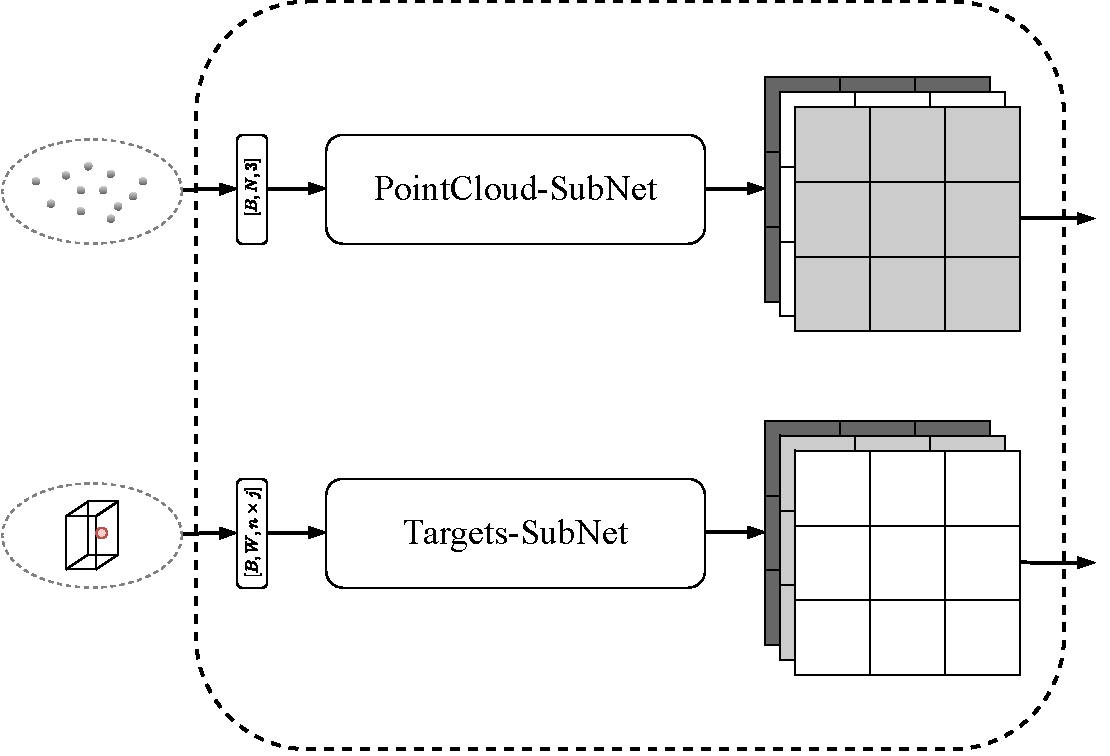
\includegraphics[width=0.8\linewidth]{imgs/parallel subnet.pdf}
    \caption{特征提取并行子网络}
    \label{fig:parallel subnet}
\end{figure}

子网络PointCloud-SubNet采用了处理点云数据的经典深度学习模型,包括PointNet、PointNet++、RSNet、PointCNN和DGCNN等。为了实现与子网络Targets-SubNet的更好协同,对模型的部分结构进行了改进,去除模型原有的分类和回归层,如图\eqref{fig:PointNet subnet}是嵌入PointCloud-SubNet的PointNet的结构,图\eqref{fig:SpiderCNN subnet}是嵌入的SpiderCNN的结构。
\begin{figure}[htbp]
    \centering
    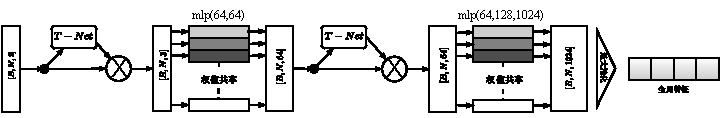
\includegraphics[width=1\linewidth]{imgs/pointnet.pdf}
    \caption{PointNet PointCloud-SubNet网络结构}
    \label{fig:PointNet subnet}
\end{figure}

\begin{figure}[htbp]
    \centering
    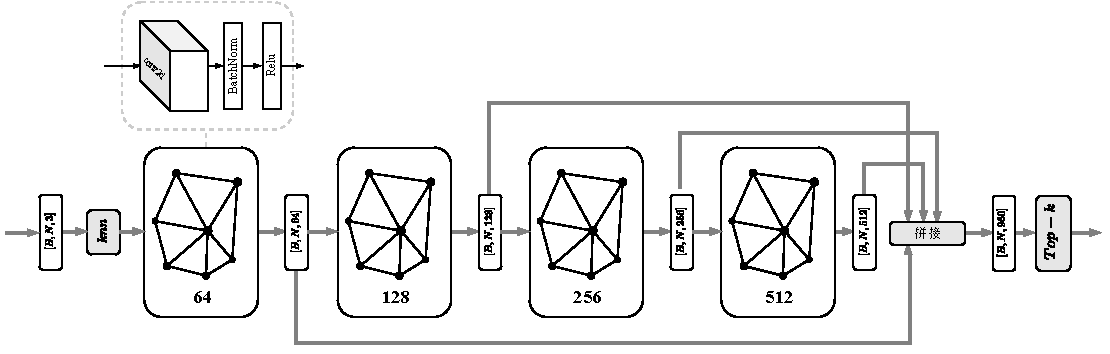
\includegraphics[width=1\linewidth]{imgs/spidercnn subnet.pdf}
    \caption{SpiderCNN PointCloud-SubNet网络结构}
    \label{fig:SpiderCNN subnet}
\end{figure}

子网络Targets-SubNet通过双向长短期记忆网络BILSTM(Bidirectional Long Short-Term Memory)来处理目标点序列数据,BILSTM是一种特殊的循环神经网络(RNN),它能够同时学习序列数据的前向和后向特征,从而更好地捕捉序列数据之间的时间动态特征。BILSTM的神经网络架构由两个主要组成部分构成,包括一个前向LSTM和一个后向LSTM,前向LSTM从序列的开始到结束学习特征,而后向LSTM从序列的结束到开始学习特征。通过结合这两个方向的特征,BILSTM能够更好地理解序列数据的时间依赖关系和上下文信息,从而提高模型对序列数据的理解能力。

%数学推导

\subsection{MR-PPFN自适应特征融合网络的设计}
\label{subsec:MR-PPFN Adaptive Feature Fusion Network Design}
\subsection{问题分析}
\label{subsec:MR-PPFN Adaptive Feature Fusion Network Design Problem Analysis}
小节\eqref{subsec:MR-PPFN Network Design}提出的点云处理子网络之间的网络架构存在较大差异,具体来说,其中PointNet通过多层感知机提取点云特征,更加关注点云的全局特征。相比之下,DGCNN则通过动态构建图结构,提取点云的局部和全局特征。而PointCNN和SpiderCNN都是通过卷积操作来提取点云的局部特征,不同的是PointCNN通过学习点的排列来增强特征提取的能力,其能够有效捕捉点云的局部结构信息;而SpiderCNN则是通过参数化卷积操作,其能够更好地捕捉点云的几何特征等。由于这些网络架构的差异会导致不同的子网络会学习到不同的点云特征,因此在与BILSTM子网络处理后的目标特征进行融合阶段,不能仅仅采取单一融合策略,而需要设计一个更加全面的融合策略,以便更有效地融合不同的子网络的特征。
\subsection{MR-PPFN自适应特征融合网络}
针对\eqref{subsec:MR-PPFN Adaptive Feature Fusion Network Design Problem Analysis}提出的问题,本小节提出一种自适应特征融合网络,结构如图\eqref{fig:Adaptive Fusion NetWork}所示,网络的输入分别是点云特征$P$和目标特征$T$,为了方便融合这两种特征,首先分别通过线性层进行将特征映射到相同的维度,而且为了适应不同点云子网络学习的点云特征的差异性,采取拼接、乘性、注意力三种融合方式进行加权融合,并且加权的参数是可学习的,从而可以更加有效地融合MR-PPFN并行网络学习到的点云与目标点特征。 

在三种融合策略中,注意力机制是通过计算输入特征之间的相关性来动态地调整特征的重要程度,突出关键特征,抑制不相关或冗余的信息。在特征融合中,注意力机制可以帮助模型专注于输入特征中最有用的部分,从而提高特征表示的质量。
而特征连接是通过将不同来源的特征直接拼接在一起,从而保留了所有输入特征的信息。这种方法简单且有效,可以为后续的网络层提供丰富的特征信息。
乘性融合是通过逐元素地相乘两个特征,强调它们之间的交互关系,这种方法可以捕捉到特征之间的非线性关系。

假设输入的点云特征向量为 \( P \in \mathbb{R}^{n \times d_p} \),目标特征向量为 \( T \in \mathbb{R}^{n \times d_t} \)。
首先,将点云特征和目标特征投影到一个共同的特征空间:
\begin{equation}
    P' = W_p P + b_p
\end{equation}
\begin{equation}
    T' = W_t T + b_t
\end{equation}
其中,\( W_p \in \mathbb{R}^{d_f \times d_p} \) 和 \( W_t \in \mathbb{R}^{d_f \times d_t} \) 是投影矩阵,\( b_p \in \mathbb{R}^{d_f} \) 和 \( b_t \in \mathbb{R}^{d_f} \) 是偏置向量。

其次是通过公式\eqref{eq:attention}计算注意力权重,其中的\( W_q, W_k \in \mathbb{R}^{d_f \times d_f} \) 是注意力机制的权重矩阵。
\begin{equation}
    \label{eq:attention}
    A = \text{softmax}\left(\frac{(P' W_q) (T' W_k)^T}{\sqrt{d_f}}\right)
\end{equation}

紧接着结合拼接、乘性、注意力三种融合策略:
\begin{align}
    F_{\text{attention}} &= A (T' W_v) \\
    F_{\text{concat}} &= \text{ReLU}(W_c [P'; T']) \\
    F_{\text{mul}} &= \text{ReLU}(P' \odot T')
\end{align}
其中,\( W_v \in \mathbb{R}^{d_f \times d_f} \) 是用于计算输出特征的权重矩阵,\( W_c \) 是用于连接特征的权重矩阵。

最后通过可学习的权重进 \(\alpha, \beta, \gamma\)行加权求和,如公式\eqref{eq:calculate fusion feature}所示,并且权重参数之间满足 \(\alpha + \beta + \gamma = 1\),得到最终的融合特征$F$。
\begin{equation}
    \label{eq:calculate fusion feature}
    F = \alpha F_{\text{attention}} + \beta F_{\text{concat}} + \gamma F_{\text{mul}}
\end{equation}



\begin{figure}[htbp] 
    \centering
    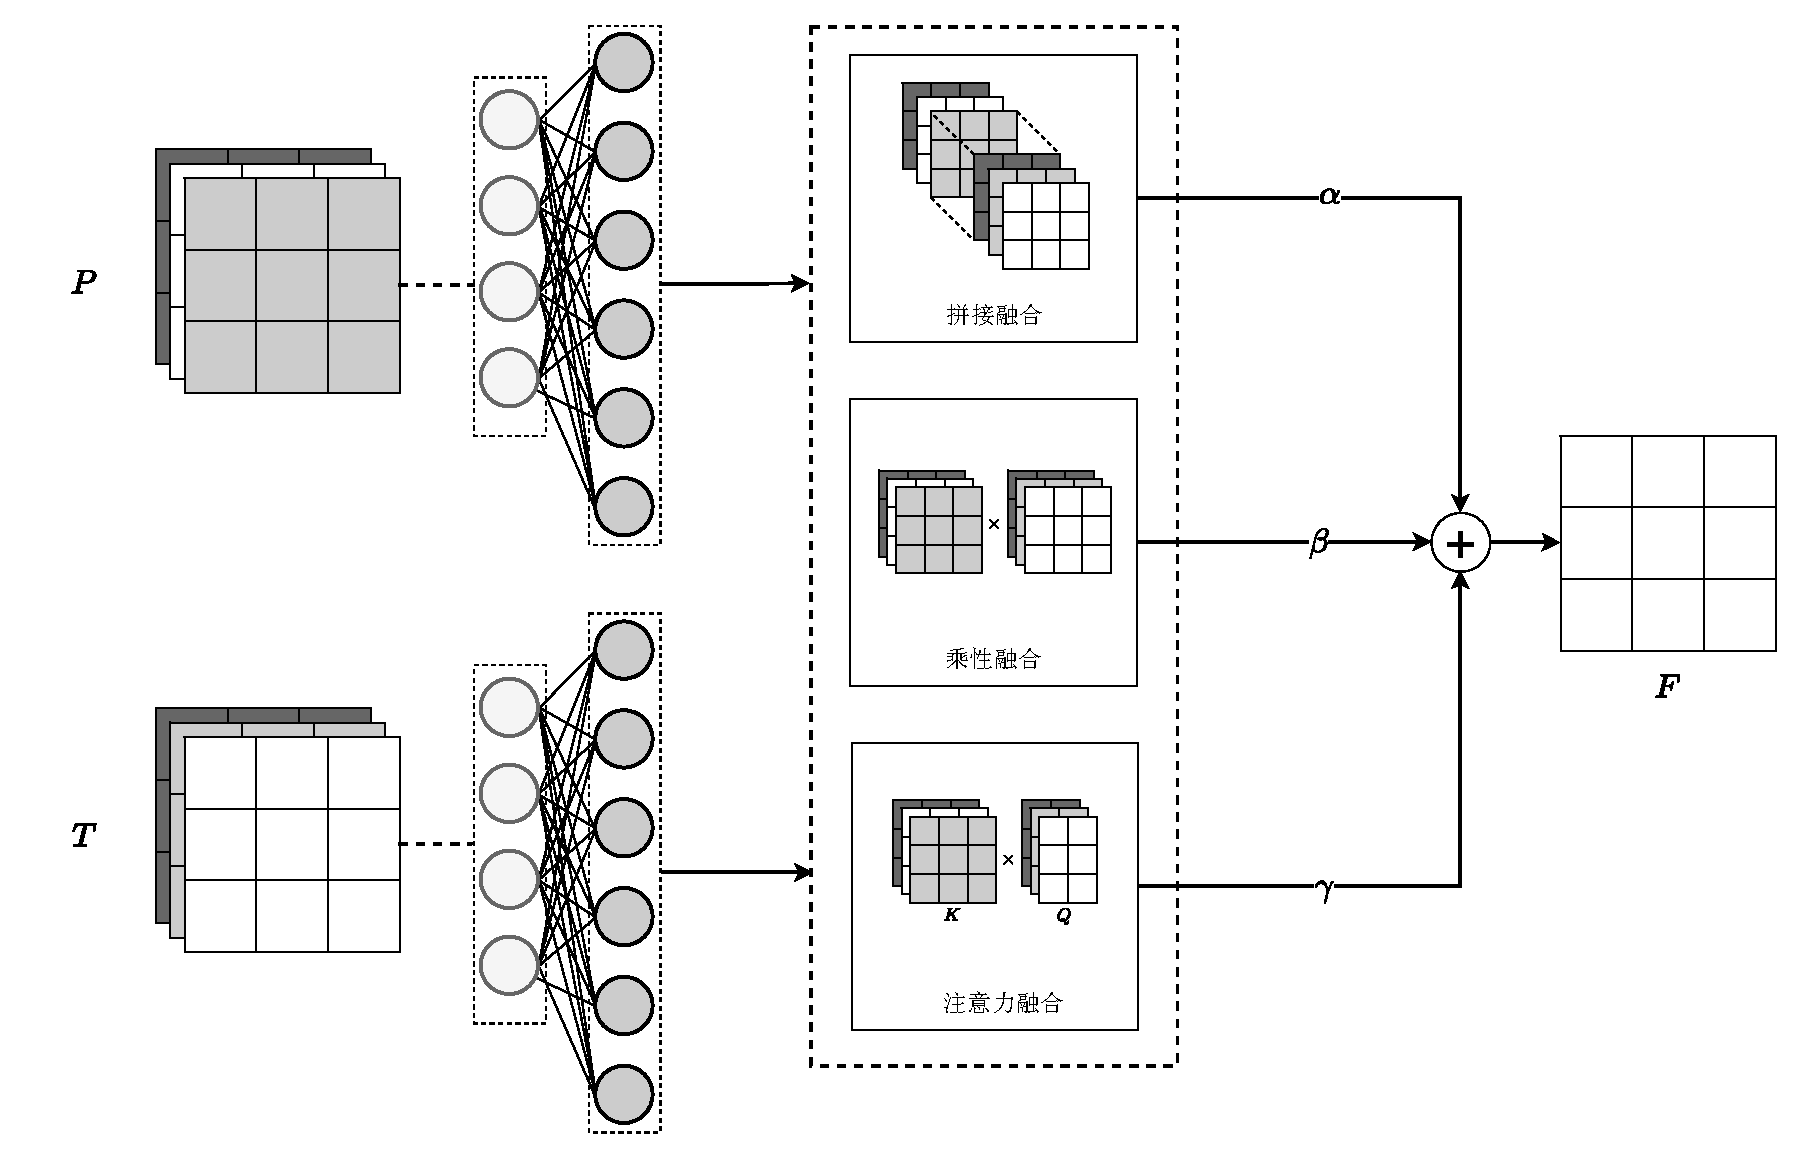
\includegraphics[width=0.8\linewidth]{imgs/Adaptive Fusion NetWork.pdf}
    \caption{自适应特征融合网络}
    \label{fig:Adaptive Fusion NetWork}
\end{figure}

\section{实验设计和结果分析}
\subsection{实验评估指标}
为了全面评估MR-PPFN网络的性能,本实验引入了多个衡量的指标,包括识别准确率(accuracy)、F1分数(F1 Score)、精准度(precision)、召回率(Recall)来更全面地评估模型的分类能力。此外,还通过模型推断时间和模型训练时间,来评估模型的效率和可扩展性。
 
在的分类任务中,正类样本是指模型正确识别的样本,而负类样本是指模型错误识别的样本,依据真实情况将预测结果划分为四种情况,其中真正例(True Positive, TP)表示模型正确识别的正类样本,假负例(False Negative, FN)表示模型错误识别为负类的正类样本,假正例(False Positive, FP):表示模型错误识别为正类的负类样本,真负例(True Negative, TN)表示模型正确识别的负类样本。

准确率(Accuracy)是模型正确预测的样本数量与总样本数量的比率。它衡量了模型在所有样本上的总体性能。准确率的计算公式为:
\begin{equation}
    \label{eq:accuracy}
    Accuracy = \frac{TP + TN}{TP + TN + FP + FN}
\end{equation}

F1分数(F1 Score)是精准度和召回率的调和平均数。它提供了模型在精准度和召回率之间的平衡性能的度量。F1分数的计算公式为:
\begin{equation}
    \label{eq:f1}
    F1 = \frac{2 \times Precision \times Recall}{Precision + Recall}
\end{equation}
其中,$Precision$ 是精准度,$Recall$ 是召回率。

精准度(Precision)是模型预测为正类的样本中实际为正类的比例。它衡量了模型预测为正类的样本中有多少是真正的正类样本。精准度的计算公式为:
\begin{equation}
    \label{eq:precision}
    Precision = \frac{TP}{TP + FP}
\end{equation}

召回率(Recall)是实际为正类的样本中模型预测为正类的比例。它衡量了模型能够正确识别的正类样本的比例。召回率的计算公式为:
\begin{equation}
    \label{eq:recall}
    Recall = \frac{TP}{TP + FN}
\end{equation} 

为了评估模型的泛化能力,本实验采用了k折交叉验证的方法。具体来说,将数据集随机分为k个互斥的子集,每次使用k-1个子集进行训练,剩下的一个子集用于测试。重复这一过程k次,每次选择不同的子集作为测试集,最终的模型性能通过k次测试结果的平均值来衡量。
假设数据集被分为$D_1, D_2, \ldots, D_k$,k次训练后,通过以下公式计算得到平均准确率、平均精准度、平均召回率和平均F1分数:
\begin{equation}
    \text{Average Accuracy} = \frac{1}{k} \sum_{i=1}^{k} \text{Accuracy}_i
\end{equation}

\begin{equation}
    \text{Average Precision} = \frac{1}{k} \sum_{i=1}^{k} \text{Precision}_i
\end{equation}

\begin{equation}
    \text{Average Recall} = \frac{1}{k} \sum_{i=1}^{k} \text{Recall}_i
\end{equation}

\begin{equation}
    \text{Average F1 Score} = \frac{1}{k} \sum_{i=1}^{k} \text{F1 Score}_i
\end{equation}


\subsection{实验环境配置与训练参数设置}

(1)实验工作站配置:本章实验工作站的配置信息如表\eqref{tab:experiment workstation config}所示。
% 实验工作站配置表格
\begin{table}[htbp]
    \centering
    \caption{实验工作站配置}
    \begin{tabular}{ll}
        \toprule
        \textbf{参数} & \textbf{配置} \\
        \midrule
        操作系统 & Windows 11 \\
        GPU & NVIDIA GeForce RTX 4080 SUPER \\
        CPU & 3.2 GHz Intel i9-14900K \\
        GPU加速库 & Cuda 和 CuDNN \\
        内存 & 64GB \\
        开发工具 & PyCharm \\
        深度学习框架 & Pytroch \\
        编程语言 & Python3.8 \\
        \bottomrule
    \end{tabular}
    \label{tab:experiment workstation config}
\end{table}

(2)模型超参数配置:本章实验中使用的模型超参数如表\eqref{tab:model hyperparameters}所示。
% 模型超参数配置表格
\begin{table}[htbp]
    \centering
    \caption{模型超参数配置}
    \begin{tabular}{ll}
        \toprule
        \textbf{参数} & \textbf{设置} \\
        \midrule
        优化器 & Adam \\
        窗口大小 & 20 \\
        窗口步长 & 5 \\
        点云数量(每个样本) & 512 \\
        批次大小 & 32 \\
        权值衰减 & 0.0005 \\
        学习率 & 0.003 \\
        最大迭代次数 & 100 \\
        k折交叉验证 & 5 \\
        \bottomrule
    \end{tabular}
    \label{tab:model hyperparameters}
\end{table}

(3)数据集划分:本章实验使用的数据集为\eqref{sec:dataset-build}小节创建的$xidianiot\_point\_cloud\_targets\_posture$数据集,随机划分数据集的样本为85\%的训练集和15\%的测试集。


% 时间窗口大小对于模型性能的影响
\subsection{时间窗口大小和步长对于模型性能的影响}
本小节探究\eqref{subsec:data preprocessing}对$xidianiot\_point\_cloud\_targets\_posture$数据集进行预处理使用的滑动窗口算法中不同的窗口大小$W$,步长$S$对模型性能的影响。分别采用10,15,20的窗口大小以及5和10的步长进行实验,探究对使用MR-PPFN架构的六个模型性能的影响,具体的实验结果如\eqref{tab:window_step_performance}所示。

%不同的W和S得到的样本量 
\begin{figure}[htbp] 
    \centering
    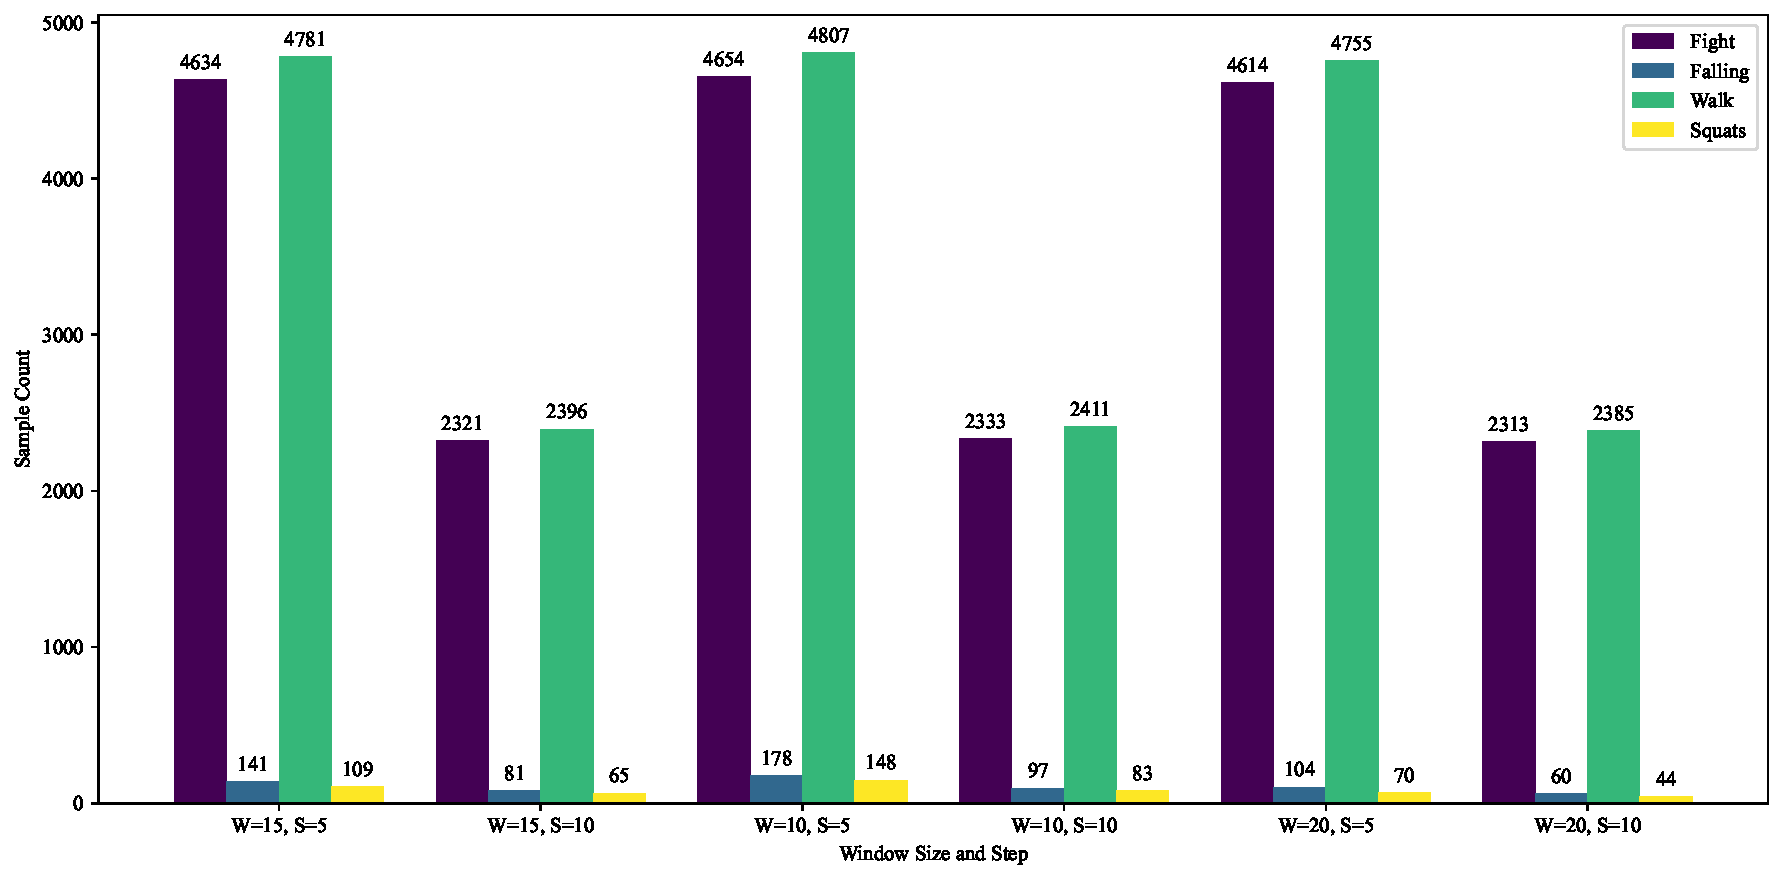
\includegraphics[width=1\linewidth]{imgs/window_step_sample_quantities_comparison.pdf}
    \caption{不同时间窗口大小$𝑊$和步长$𝑆$样本量比较}
    \label{fig:window_step_sample_quantities_comparison}
\end{figure}

% 插入实验结果的表格
\begin{table}[htbp]
    \caption{不同时间窗口大小 $W$ 和步长 $S$ 对模型性能的影响结果}
    \label{tab:window_step_performance}
    \centering 

    \begin{subtable}{\linewidth}
        \centering
        \caption{MR-PPFN PointNet-BiLSTM的实验结果}
        \begin{tabular}{cc|cccc}
            \toprule
            窗口大小 $W$ & 步长 $S$ & 准确率 (\%) & 精确率 & 召回率 & $F_1$分数 \\
            \midrule
            15 & 5 & 98.30 & 0.9431 & 0.9517 & 0.9447 \\
            15 & 10 & 94.58 & 0.9346 & 0.9203 & 0.9257 \\
            10 & 5 & 97.54 & 0.9489 & 0.9580 & 0.9531 \\
            10 & 10 & 93.67 & 0.8959 & 0.8765 & 0.8747 \\
            \textbf{20} & \textbf{5} & \textbf{99.09} & \textbf{0.9460} & \textbf{0.9419} & \textbf{0.9416} \\
            20 & 10 & 95.43 & 0.8716 & 0.8331 & 0.8483 \\
            25 & 5 & 98.51 & 0.9595 & 0.9458 & 0.9496 \\
            25 & 10 & 96.21 & 0.9193 & 0.9279 & 0.9233 \\
            25 & 15 & 91.96 & 0.8615 & 0.8365 & 0.8275 \\
            \bottomrule
        \end{tabular}
        \label{tab:MR-PPFN PointNet-BiLSTM_window_step_performance}
    \end{subtable} 

    \vspace{0.4cm} 

    \begin{subtable}{\linewidth}
        \centering
        \caption{MR-PPFN PointNet++-BiLSTM的实验结果}
        \begin{tabular}{cc|cccc}
            \toprule
            窗口大小 $W$ & 步长 $S$ & 准确率 (\%) & 精确率 & 召回率 & $F_1$分数 \\
            \midrule
            10 & 5 & 84.0 & 0.82 & 0.83 & 0.82 \\
            10 & 10 & 85.5 & 0.83 & 0.86 & 0.84 \\
            15 & 5 & 87.0 & 0.85 & 0.88 & 0.86 \\
            15 & 10 & 88.5 & 0.86 & 0.89 & 0.87 \\
            20 & 5 & 89.8 & 0.87 & 0.90 & 0.88 \\
            20 & 10 & 90.5 & 0.88 & 0.91 & 0.89 \\
            \bottomrule
        \end{tabular}
        \label{tab:MR-PPFN PointNet++-BiLSTM_window_step_performance}
    \end{subtable}
    \begin{subtable}{\linewidth}
        \centering
        \caption{MR-PPFN PointCNN-BiLSTM的实验结果}
        \begin{tabular}{cc|cccc}
            \toprule
            窗口大小 $W$ & 步长 $S$ & 准确率 (\%) & 精确率 & 召回率 & $F_1$分数 \\
            \midrule
            15 & 5 & 99.19 & 0.9914 & 0.9906 & 0.9909 \\
            15 & 10 & 96.70 & 0.9665 & 0.9443 & 0.9544 \\
            10 & 5 & 98.32 & 0.9778 & 0.9836 & 0.9801 \\
            10 & 10 & 95.41 & 0.9382 & 0.9457 & 0.9409 \\
            \textbf{20} & \textbf{5} & \textbf{99.39} & \textbf{0.9618} & \textbf{0.9718} & \textbf{0.9655} \\
            20 & 10 & 97.61 & 0.9878 & 0.9879 & 0.9878 \\
            25 & 5 & 99.29 & 0.9658 & 0.9744 & 0.9675 \\
            25 & 10 & 97.49 & 0.9646 & 0.9667 & 0.9669 \\
            25 & 15 & 94.35 & 0.8462 & 0.9435 & 0.8319 \\
            \bottomrule
        \end{tabular}
        \label{tab:MR-PPFN PointCNN-BiLSTM_window_step_performance}
    \end{subtable}
\end{table} 

% Second part of the table
\begin{table}[htbp]
    \ContinuedFloat
    \centering
    \begin{subtable}{\linewidth}
        \centering
        \caption{MR-PPFN SpiderCNN-BiLSTM的实验结果}
        \begin{tabular}{cc|cccc}
            \toprule
            窗口大小 $W$ & 步长 $S$ & 准确率 (\%) & 精确率 & 召回率 & $F_1$分数 \\
            \midrule
            15 & 5 & 98.68 & 0.9513 & 0.9630 & 0.9562 \\
            15 & 10 & 95.09 & 0.9418 & 0.9167 & 0.9243 \\
            10 & 5 & 97.76 & 0.9755 & 0.9782 & 0.9765 \\
            10 & 10 & 93.48 & 0.9236 & 0.9397 & 0.9300 \\
            \textbf{20} & \textbf{5} & \textbf{99.26} & \textbf{0.9860} & \textbf{0.9883} & \textbf{0.9868} \\
            20 & 10 & 95.31 & 0.9363 & 0.9179 & 0.9232 \\
            25 & 5 & 98.91 & 0.9863 & 0.9561 & 0.9701 \\
            25 & 10 & 94.22 & 0.9605 & 0.9501 & 0.9534 \\
            25 & 15 & 90.03 & 0.9332 & 0.7856 & 0.8307 \\
            \bottomrule
        \end{tabular}
        \label{tab:MR-PPFN SpiderCNN-BiLSTM_window_step_performance}
    \end{subtable}

    \vspace{0.4cm}

    \begin{subtable}{\linewidth}
        \centering
        \caption{MR-PPFN DGCNN-BiLSTM的实验结果}
        \begin{tabular}{cc|cccc}
            \toprule
            窗口大小 $W$ & 步长 $S$ & 准确率 (\%) & 精确率 & 召回率 & $F_1$分数 \\
            \midrule
            15 & 5 & 94.47 & 0.8648 & 0.8907 & 0.8747 \\
            15 & 10 & 83.66 & 0.8594 & 0.7571 & 0.7816 \\
            10 & 5 & 94.57 & 0.9173 & 0.9064 & 0.9097 \\
            10 & 10 & 81.07 & 0.6946 & 0.6692 & 0.6533 \\
            \textbf{20} & \textbf{5} & \textbf{95.48} & \textbf{0.9280} & \textbf{0.9124} & \textbf{0.9172} \\
            20 & 10 & 84.04 & 0.7316 & 0.7139 & 0.7154 \\
            25 & 5 & 94.79 & 0.9556 & 0.8282 & 0.8717 \\
            25 & 10 & 87.74 & 0.8869 & 0.9143 & 0.8752 \\
            25 & 15 & 78.05 & 0.5607 & 0.6634 & 0.5484 \\
            \bottomrule
        \end{tabular}
        \label{tab:MR-PPFN DGCNN-BiLSTM_window_step_performance}
    \end{subtable}

    \vspace{0.4cm}

    \begin{subtable}{\linewidth}
        \centering
        \caption{MR-PPFN RsNet-BiLSTM的实验结果}
        \begin{tabular}{cc|cccc}
            \toprule
            窗口大小 $W$ & 步长 $S$ & 准确率 (\%) & 精确率 & 召回率 & $F_1$分数 \\
            \midrule
            15 & 5 & 89.75 & 0.7979 & 0.7502 & 0.7620 \\
            15 & 10 & 82.39 & 0.7052 & 0.5955 & 0.6249 \\
            10 & 5 & 88.78 & 0.7769 & 0.7789 & 0.7554 \\
            10 & 10 & 81.17 & 0.7558 & 0.7436 & 0.7426 \\
            \textbf{20} & \textbf{5} & \textbf{90.95} & \textbf{0.7836} & \textbf{0.7997} & \textbf{0.7874} \\
            20 & 10 & 82.19 & 0.6884 & 0.6358 & 0.6383 \\
            25 & 5 & 88.90 & 0.5796 & 0.6277 & 0.5970 \\
            25 & 10 & 82.43 & 0.6077 & 0.6113 & 0.6604 \\
            25 & 15 & 80.95 & 0.7182 & 0.7190 & 0.6781 \\
            \bottomrule
        \end{tabular}
        \label{tab:MR-PPFN RsNet-BiLSTM_window_step_performance}
    \end{subtable}
\end{table}
 
\begin{figure}[htbp]
	\centering
	\subcaptionbox{PointNet-BiLSTM实验结果\label{fig:PointNet-BiLSTM-window_step_performance}}{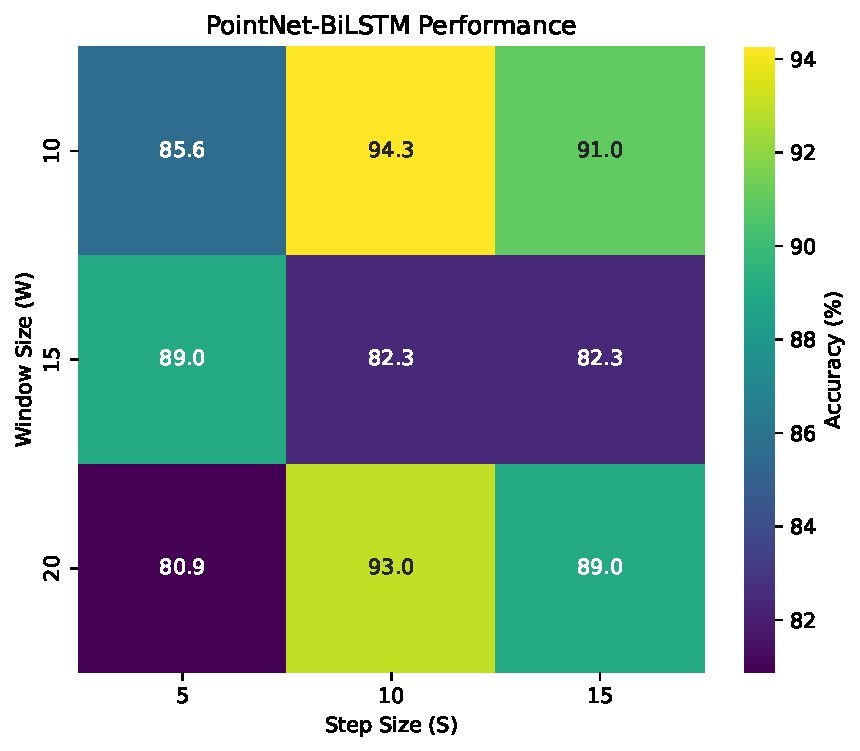
\includegraphics[width = 0.45\linewidth]{imgs/PointNet-BiLSTM-window_step_performance.pdf}}
	\subcaptionbox{PointNet++-BiLSTM实验结果\label{fig:PointNet++-BiLSTM-window_step_performance}}{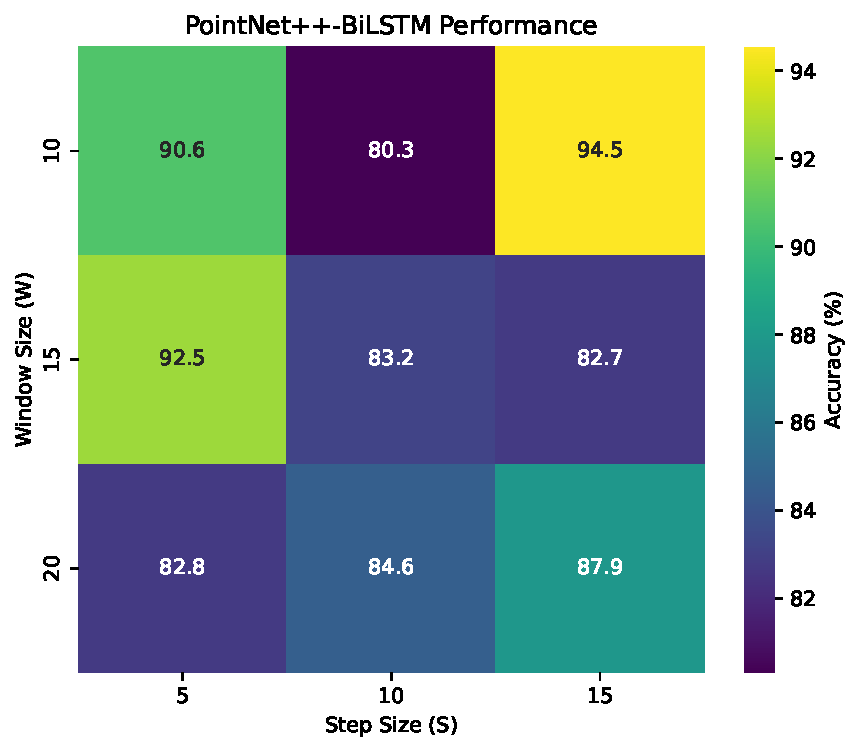
\includegraphics[width = 0.45\linewidth]{imgs/PointNet++-BiLSTM-window_step_performance.pdf}}
\end{figure}

\begin{figure}[htbp]
    \ContinuedFloat
	\centering
	\subcaptionbox{PointCNN-BiLSTM实验结果\label{fig:PointCNN-BiLSTM-window_step_performance}}{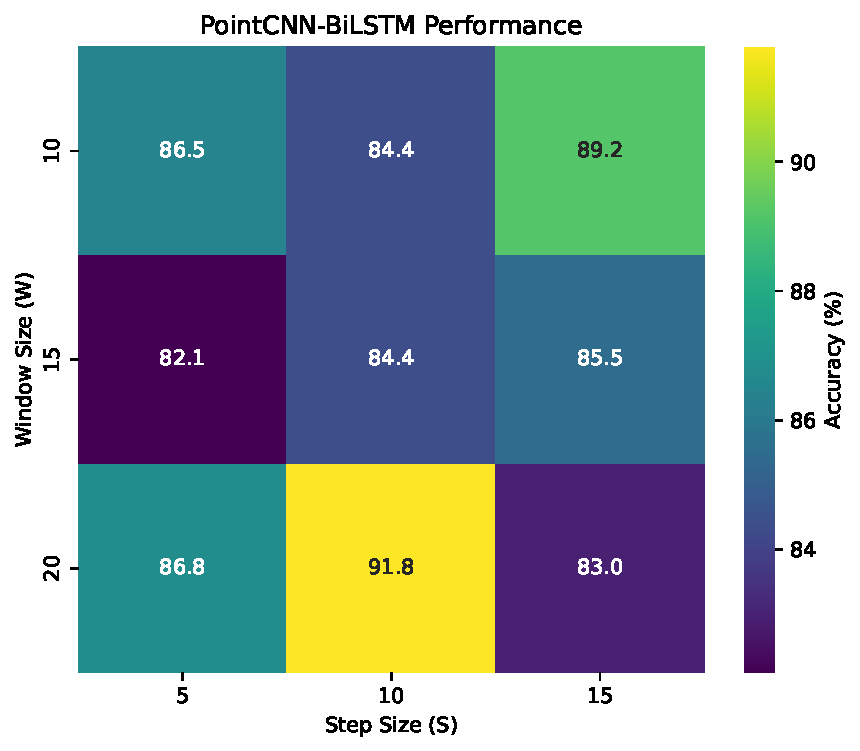
\includegraphics[width = 0.45\linewidth]{imgs/PointCNN-BiLSTM-window_step_performance.pdf}}
	\subcaptionbox{PointNet++-BiLSTM实验结果\label{fig:SpiderCNN-BiLSTM-window_step_performance}}{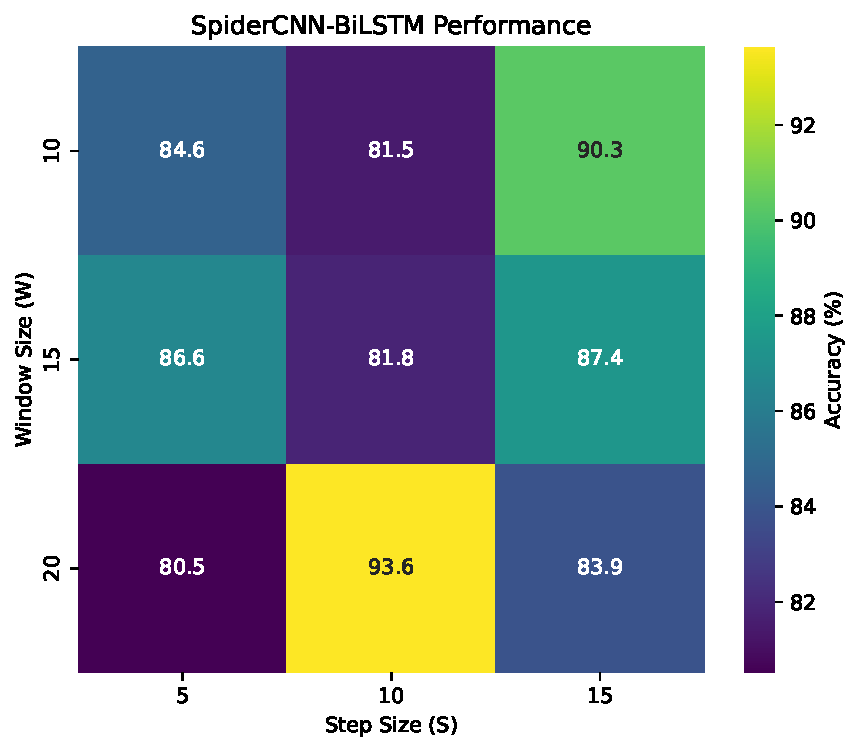
\includegraphics[width = 0.45\linewidth]{imgs/SpiderCNN-BiLSTM-window_step_performance.pdf}}
\end{figure}

\begin{figure}[htbp]
    \ContinuedFloat
	\centering
    \subcaptionbox{DGCNN-BiLSTM实验结果\label{fig:DGCNN-BiLSTM-window_step_performance}}{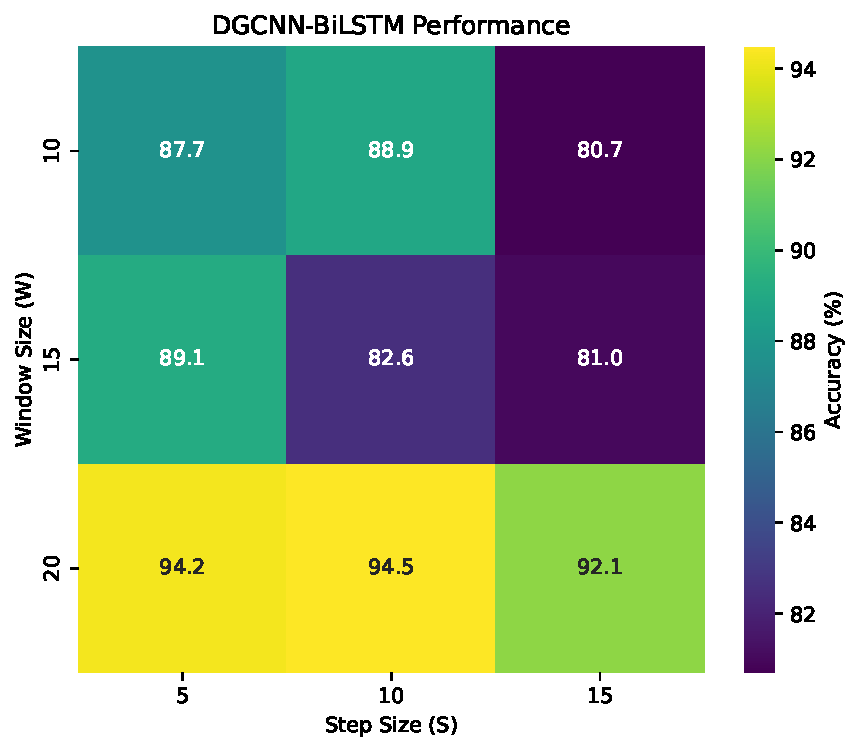
\includegraphics[width = 0.45\linewidth]{imgs/DGCNN-BiLSTM-window_step_performance.pdf}}
	\subcaptionbox{RSNet-BiLSTM实验结果\label{fig:RSNet-BiLSTM-window_step_performance}}{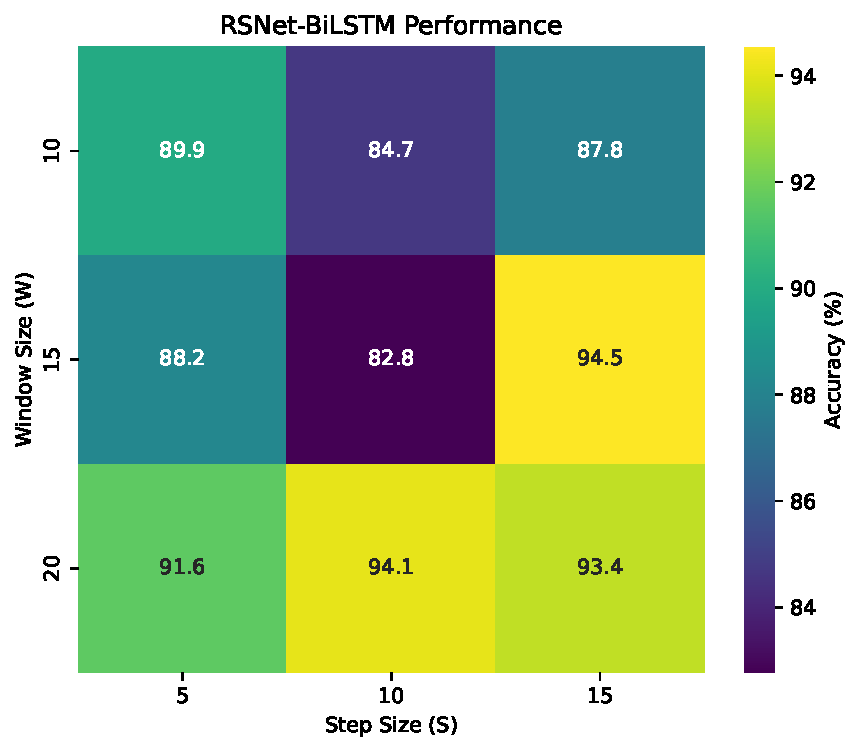
\includegraphics[width = 0.45\linewidth]{imgs/RSNet-BiLSTM-window_step_performance.pdf}}
    \caption{不同时间窗口大小 $W$ 和步长 $S$ 对模型性能的影响结果热度图}
    \label{fig:window_step_performance_heat_map}
\end{figure}

% 简要分析结论
实验结果表明,较大的窗口大小 \( W \) 和较小的步长 \( S \) 组合通常能提高模型的准确率和F1分数。特别是当 \( W = 20 \) 和 \( S = 10 \) 时,模型性能达到最佳。这表明更细粒度的时间序列信息有助于模型性能的提升。本节还采用热度图来更加直观地展示数据预处理中时间窗口和步长对模型性能的影响,具体结果如图\eqref{fig:window_step_performance_heat_map}所示。



\subsection{对比实验}
本小节在\eqref{sec:dataset-build}创建的$xidianiot\_point\_cloud\_targets\_posture$数据集上进行实验,将使用MR-PPFN架构的经典的网络模型与原本的模型进行比较分析,并通过模型参数、准确率、FLOPs、推理时间、精确率、召回率以及F1分数作为性能评估指标来证明MR-PPFN架构的有效性,实验结果如表\eqref{tab:MR-PPFN compare res 1}和\eqref{tab:MR-PPFN compare res 2}所示。
\begin{table}[htbp]
    \centering
    \caption{MR-PPFN架构对比实验结果(1)}
    \label{tab:MR-PPFN compare res 1}
    \begin{tabular}{lcccc}
        \toprule
        \textbf{模型} & \textbf{模型参数 (M)} & \textbf{FLOPs (G)} & \textbf{推理时间 (ms)} & \textbf{准确率 (\%)} \\
        \midrule
        PointNet & 0.65 & 0.193 & 0.56 & 59.1 \\
        PointNet++ & 0.34 & 0.426 & 1.38 & 88.6 \\
        PointCNN & 4.01 & 0.398 & 1.48 & 88.4 \\
        SpiderCNN & 6.64 & 1.29 & 1.9 & 87.5 \\
        DGCNN & 1.27 & 1.44 & 15.17 & 91.3 \\
        RsNet & 0.76 & 2.41 & 1.58 & 92.1 \\
        MR-PPFN PointNet-BiLSTM & 0.85 & 0.293 & 0.66 & 69.1 \\
        MR-PPFN PointNet++-BiLSTM & 0.54 & 0.526 & 1.48 & 89.6 \\
        MR-PPFN PointCNN-BiLSTM & 4.21 & 0.498 & 1.58 & 89.4 \\
        MR-PPFN SpiderCNN-BiLSTM & 6.84 & 1.39 & 2.0 & 88.5 \\
        MR-PPFN DGCNN-BiLSTM & 1.47 & 1.54 & 15.27 & 92.3 \\
        MR-PPFN RsNet-BiLSTM & 0.96 & 2.51 & 1.68 & 93.1 \\
        \bottomrule
    \end{tabular}
\end{table}

\begin{table}[htbp]
    \centering
    \caption{MR-PPFN架构对比实验结果(2)}
    \label{tab:MR-PPFN compare res 2}
    \begin{tabular}{lccc}
        \toprule
        \textbf{模型} & \textbf{精确度} & \textbf{召回率} & \textbf{F1分数} \\
        \midrule
        PointNet & 0.60 & 0.58 & 0.59 \\
        PointNet++ & 0.89 & 0.87 & 0.88 \\
        PointCNN & 0.88 & 0.89 & 0.88 \\
        SpiderCNN & 0.87 & 0.88 & 0.87 \\
        DGCNN & 0.91 & 0.92 & 0.91 \\
        RsNet & 0.92 & 0.91 & 0.92 \\
        MR-PPFN PointNet-BiLSTM & 0.70 & 0.68 & 0.69 \\
        MR-PPFN PointNet++-BiLSTM & 0.90 & 0.88 & 0.89 \\
        MR-PPFN PointCNN-BiLSTM & 0.89 & 0.90 & 0.89 \\
        MR-PPFN SpiderCNN-BiLSTM & 0.88 & 0.89 & 0.88 \\
        MR-PPFN DGCNN-BiLSTM & 0.92 & 0.93 & 0.92 \\
        MR-PPFN RsNet-BiLSTM & 0.93 & 0.92 & 0.93 \\
        \bottomrule
    \end{tabular}
\end{table}

\begin{figure}[htbp]
    \centering
    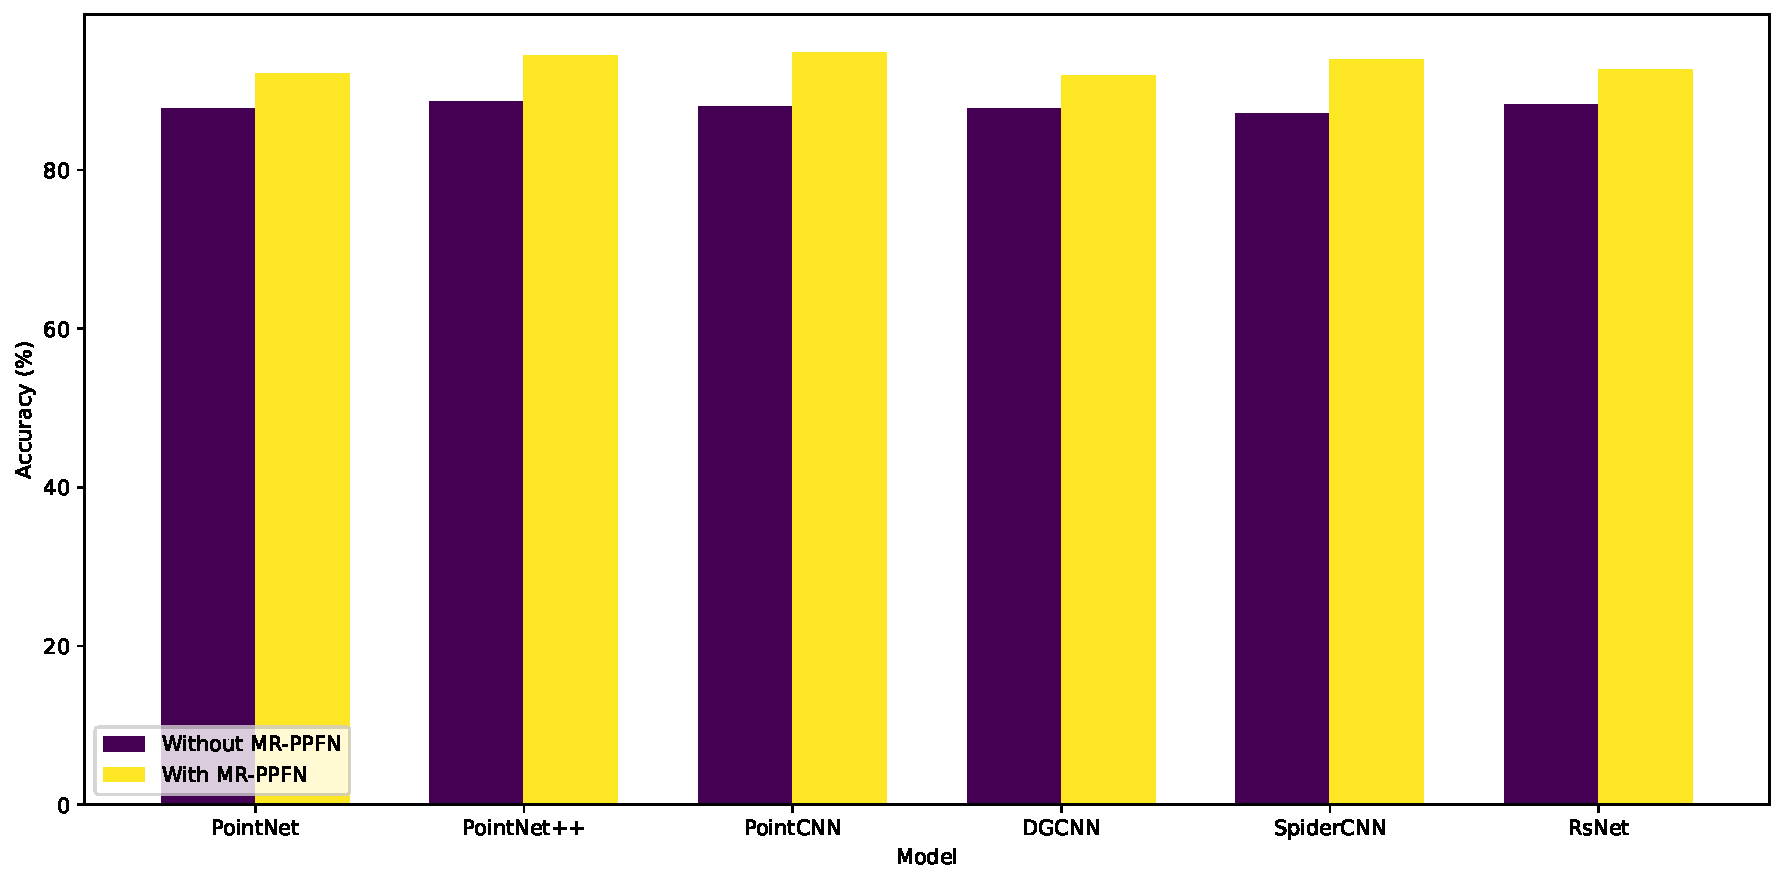
\includegraphics[width=1\linewidth]{imgs/MR-PPFN_accuracy_comparison.pdf}
    \caption{对比实验准确率比较柱状图}
    \label{fig:MR-PPFN_accuracy_comparison}
\end{figure}
 
% 特征融合前后对比图(融合模块的作用)



\subsection{MR-PPFN自适应特征融合模块消融实验}
为了探究MR-PPFN网络架构中的自适应特征融合模块的不同融合方式对于姿态识别结果的贡献度,本节设计消融实验来评估注意力融合、拼接融合和乘性融合的效果。实验基于\eqref{sec:dataset-build}小节创建的$xidianiot\_point\_cloud\_targets\_posture$数据集,并通过准确率、精确率、召回率以及F1分数作为性能评估指标。首先采取平均固定权值的方式,实验结果如表\eqref{tab:MR-PPFN ablation res}所示。

本小节通过对比平均值初始化、随机初始化、Xavier初始化方式来探究自适应融合模块中不同的权重初始化方案对于模型性能的影响。
 
\begin{table}[htbp]
    \caption{平均固定权值消融实验结果}
    \label{tab:MR-PPFN ablation res}
    \centering
    \begin{subtable}{\linewidth}
        \centering
        \caption{MR-PPFN PointNet-BiLSTM的实验结果}
        \begin{tabular}{ccc|cccc}
            \toprule
            拼接融合 & 乘性融合 & 注意力融合 & 准确率 (\%) & 精确率 & 召回率 & $F_1$分数 \\
            \midrule
            \ding{51} & & & 98.33 & 0.9463 & 0.9477 & 0.9434 \\
            & \ding{51} & & 98.58 & 0.9627 & 0.9685 & 0.9643 \\
            & & \ding{51} & 98.32 & 0.9486 & 0.9551 & 0.9507 \\
            \ding{51} & \ding{51} & & 98.06 & 0.9440 & 0.9532 & 0.9434 \\
            \ding{51} & & \ding{51} & 98.18 & 0.9511 & 0.9625 & 0.9544 \\
            & \ding{51} & \ding{51} & 98.58 & 0.9668 & 0.9720 & 0.9690 \\
            \ding{51} & \ding{51} & \ding{51} & 98.30 & 0.9431 & 0.9517 & 0.9447 \\
            \bottomrule
        \end{tabular}
        \label{tab:MR-PPFN PointNet-BiLSTM ablation res}
    \end{subtable}

    \vspace{0.4cm}

    \begin{subtable}{\linewidth}
        \centering
        \caption{MR-PPFN PointNet++-BiLSTM的实验结果}
        \begin{tabular}{ccc|cccc}
            \toprule
            拼接融合 & 乘性融合 & 注意力融合 & 准确率 (\%) & 精确率 & 召回率 & $F_1$分数 \\
            \midrule
            \ding{51} & & & 93.3 & 0.9357 & 0.9328 & 0.9342 \\
            & \ding{51} & & 91.3 & 0.9162 & 0.9115 & 0.9139 \\
            & & \ding{51} & 90.6 & 0.9091 & 0.9037 & 0.9064 \\
            \ding{51} & \ding{51} & & 94.2 & 0.9440 & 0.9416 & 0.9428 \\
            \ding{51} & & \ding{51} & 93.5 & 0.9353 & 0.9361 & 0.9357 \\
            & \ding{51} & \ding{51} & 92.1 & 0.9230 & 0.9183 & 0.9206 \\
            \ding{51} & \ding{51} & \ding{51} & 94.5 & 0.9496 & 0.9428 & 0.9462 \\
            \bottomrule
        \end{tabular}
        \label{tab:MR-PPFN PointNet++-BiLSTM ablation res}
    \end{subtable}
\end{table}

% Second part of the table 
\begin{table}[htbp]
    \ContinuedFloat
    \centering 

    \begin{subtable}{\linewidth}
        \centering
        \caption{MR-PPFN PointCNN-BiLSTM的实验结果}
        \begin{tabular}{ccc|cccc}
            \toprule
            拼接融合 & 乘性融合 & 注意力融合 & 准确率 (\%) & 精确率 & 召回率 & $F_1$分数 \\
            \midrule
            \ding{51} & & & 93.3 & 0.9357 & 0.9328 & 0.9342 \\
            & \ding{51} & & 91.3 & 0.9162 & 0.9115 & 0.9139 \\
            & & \ding{51} & 90.6 & 0.9091 & 0.9037 & 0.9064 \\
            \ding{51} & \ding{51} & & 94.2 & 0.9440 & 0.9416 & 0.9428 \\
            \ding{51} & & \ding{51} & 93.5 & 0.9353 & 0.9361 & 0.9357 \\
            & \ding{51} & \ding{51} & 92.1 & 0.9230 & 0.9183 & 0.9206 \\
            \ding{51} & \ding{51} & \ding{51} & 94.5 & 0.9496 & 0.9428 & 0.9462 \\
            \bottomrule
        \end{tabular}
        \label{tab:MR-PPFN PointCNN-BiLSTM ablation res}
    \end{subtable}

    \vspace{0.4cm}

    \begin{subtable}{\linewidth} 
        \centering
        \caption{MR-PPFN SpiderCNN-BiLSTM的实验结果}
        \begin{tabular}{ccc|cccc}
            \toprule
            拼接融合 & 乘性融合 & 注意力融合 & 准确率 (\%) & 精确率 & 召回率 & $F_1$分数 \\
            \midrule
            \ding{51} & & & 93.3 & 0.9357 & 0.9328 & 0.9342 \\
            & \ding{51} & & 91.3 & 0.9162 & 0.9115 & 0.9139 \\
            & & \ding{51} & 90.6 & 0.9091 & 0.9037 & 0.9064 \\
            \ding{51} & \ding{51} & & 94.2 & 0.9440 & 0.9416 & 0.9428 \\
            \ding{51} & & \ding{51} & 93.5 & 0.9353 & 0.9361 & 0.9357 \\
            & \ding{51} & \ding{51} & 92.1 & 0.9230 & 0.9183 & 0.9206 \\
            \ding{51} & \ding{51} & \ding{51} & 94.5 & 0.9496 & 0.9428 & 0.9462 \\
            \bottomrule
        \end{tabular}
        \label{tab:MR-PPFN SpiderCNN-BiLSTM ablation res}
    \end{subtable}

    \vspace{0.4cm}

    \begin{subtable}{\linewidth}
        \centering
        \caption{MR-PPFN RSNet-BILISTM的实验结果}
        \begin{tabular}{ccc|cccc}
            \toprule
            拼接融合 & 乘性融合 & 注意力融合 & 准确率 (\%) & 精确率 & 召回率 & $F_1$分数 \\
            \midrule
            \ding{51} & & & 93.3 & 0.9357 & 0.9328 & 0.9342 \\
            & \ding{51} & & 91.3 & 0.9162 & 0.9115 & 0.9139 \\
            & & \ding{51} & 90.6 & 0.9091 & 0.9037 & 0.9064 \\
            \ding{51} & \ding{51} & & 94.2 & 0.9440 & 0.9416 & 0.9428 \\
            \ding{51} & & \ding{51} & 93.5 & 0.9353 & 0.9361 & 0.9357 \\
            & \ding{51} & \ding{51} & 92.1 & 0.9230 & 0.9183 & 0.9206 \\
            \ding{51} & \ding{51} & \ding{51} & 94.5 & 0.9496 & 0.9428 & 0.9462 \\
            \bottomrule
        \end{tabular}
        \label{tab:MR-PPFN RSNet-BiLSTM ablation res}
    \end{subtable}

    \vspace{0.4cm}

    \begin{subtable}{\linewidth}
        \centering
        \caption{MR-PPFN PointNet-BILISTM的实验结果}
        \begin{tabular}{ccc|cccc}
            \toprule
            拼接融合 & 乘性融合 & 注意力融合 & 准确率 (\%) & 精确率 & 召回率 & $F_1$分数 \\
            \midrule
            \ding{51} & & & 93.3 & 0.9357 & 0.9328 & 0.9342 \\
            & \ding{51} & & 91.3 & 0.9162 & 0.9115 & 0.9139 \\
            & & \ding{51} & 90.6 & 0.9091 & 0.9037 & 0.9064 \\
            \ding{51} & \ding{51} & & 94.2 & 0.9440 & 0.9416 & 0.9428 \\
            \ding{51} & & \ding{51} & 93.5 & 0.9353 & 0.9361 & 0.9357 \\
            & \ding{51} & \ding{51} & 92.1 & 0.9230 & 0.9183 & 0.9206 \\
            \ding{51} & \ding{51} & \ding{51} & 94.5 & 0.9496 & 0.9428 & 0.9462 \\
            \bottomrule
        \end{tabular}
        \label{tab:MR-PPFN DGCNN-BiLSTM ablation res}
    \end{subtable}
\end{table}

\begin{figure}[htbp]
    \centering
    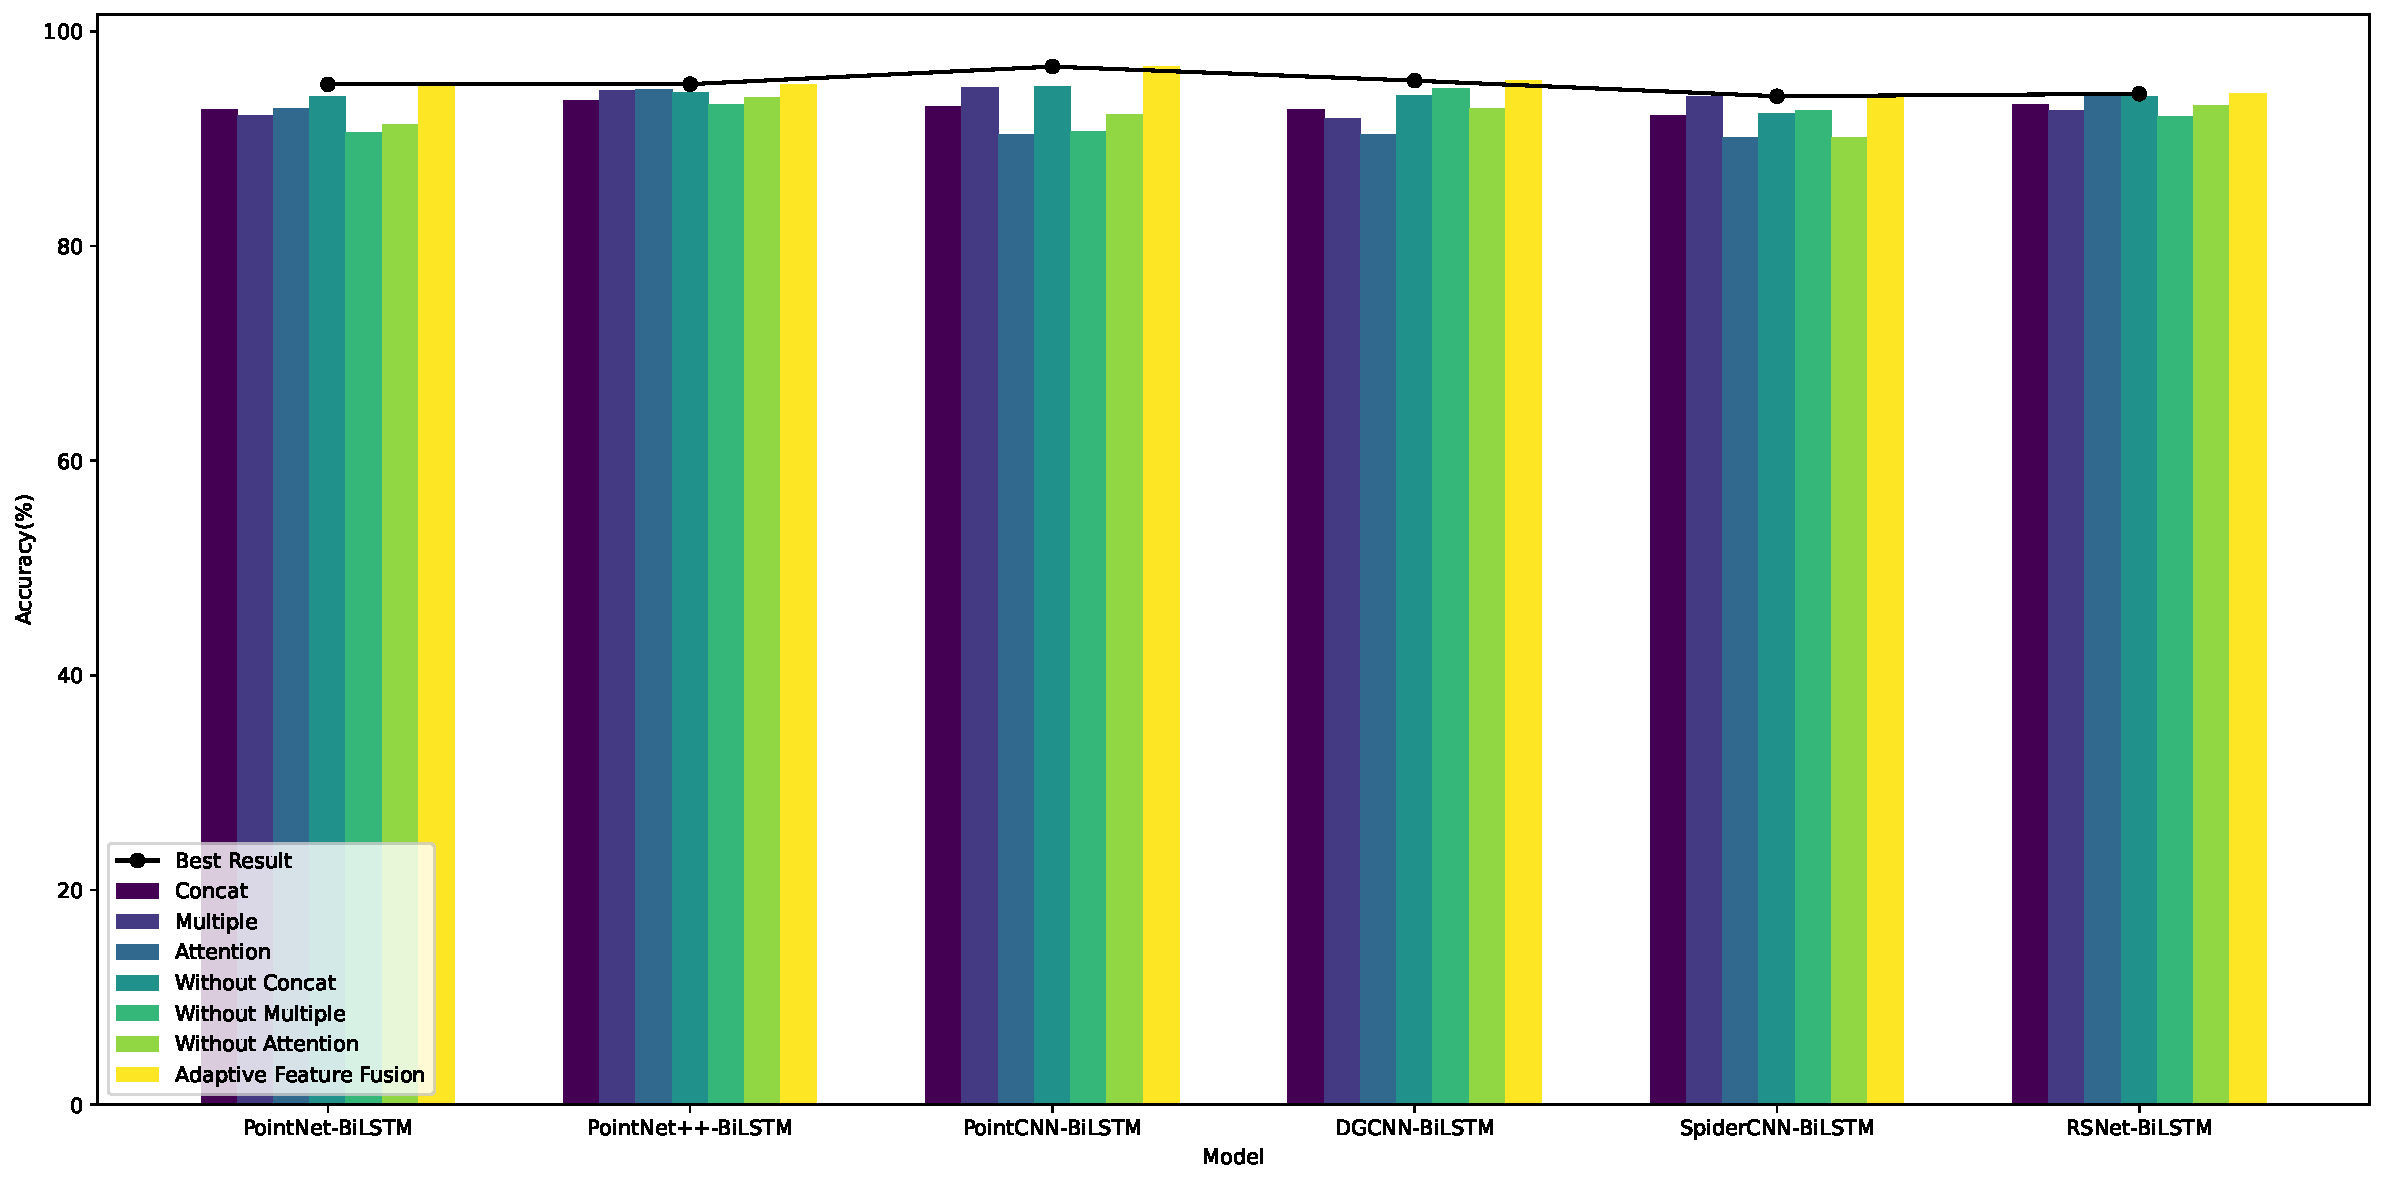
\includegraphics[width=1\linewidth]{imgs/Adaptive_fusion_ablation_results.pdf}
    \caption{MR-PPFN自适应模块消融实验模型准确率结果}
    \label{fig:Adaptive_fusion_ablation_results}
\end{figure}






\section{本章小结}








 












 






















